\documentclass[12pt]{article}
\usepackage{geometry}
\usepackage{dcolumn}
\usepackage{booktabs}
\usepackage{pdflscape}
\usepackage{graphicx}
\usepackage{placeins}
\usepackage{dcolumn}
\usepackage{xcolor}
\usepackage{booktabs}
\linespread{1.5}
\usepackage{subcaption}
\usepackage{amsmath}
\usepackage{hyperref}
\usepackage{multirow}
\usepackage[title]{appendix}
%\usepackage{xepersian}
%\settextfont{XB Zar}
%\setdigitfont{XB Zar}

\begin{document}
\nopagebreak
\newgeometry{margin = 1.2cm}
\title{
 Price Limit and Attention Grabbing \\
  \large 
 Impact of price limit hit on return, volume, and behavior of investors
  }
\author{S.Morteza Aghajanadeh}
\nopagebreak
{\maketitle}

Stocks in the Tehran Securities Exchange that hit upper price limits typically exhibit two characteristics: high
returns and high volumes. We show that these price limit events attract investors' attention.
Attention-grabbing events lead active individual investors to buy stocks.
Upper price limit events coincide with initial price increases, followed by statistically
significant price mean reversion over the following week.
 Rational traders profit in
response to attention-based buying. Smart traders accumulate shares on date t, sell shares on date t+1, and
earn an average daily profit of 3.8\%. 

Furthermore, we study the effect of the lower price hit on return and volumes. Literature often ignores this event as attention-grabbing because where investors are restricted for short selling, they do not have any selling problem. However, we show that this event can drive investors to sell their portfolios. 




\section{Probabilty of event}


\begin{landscape}
\begin{figure}
\centering
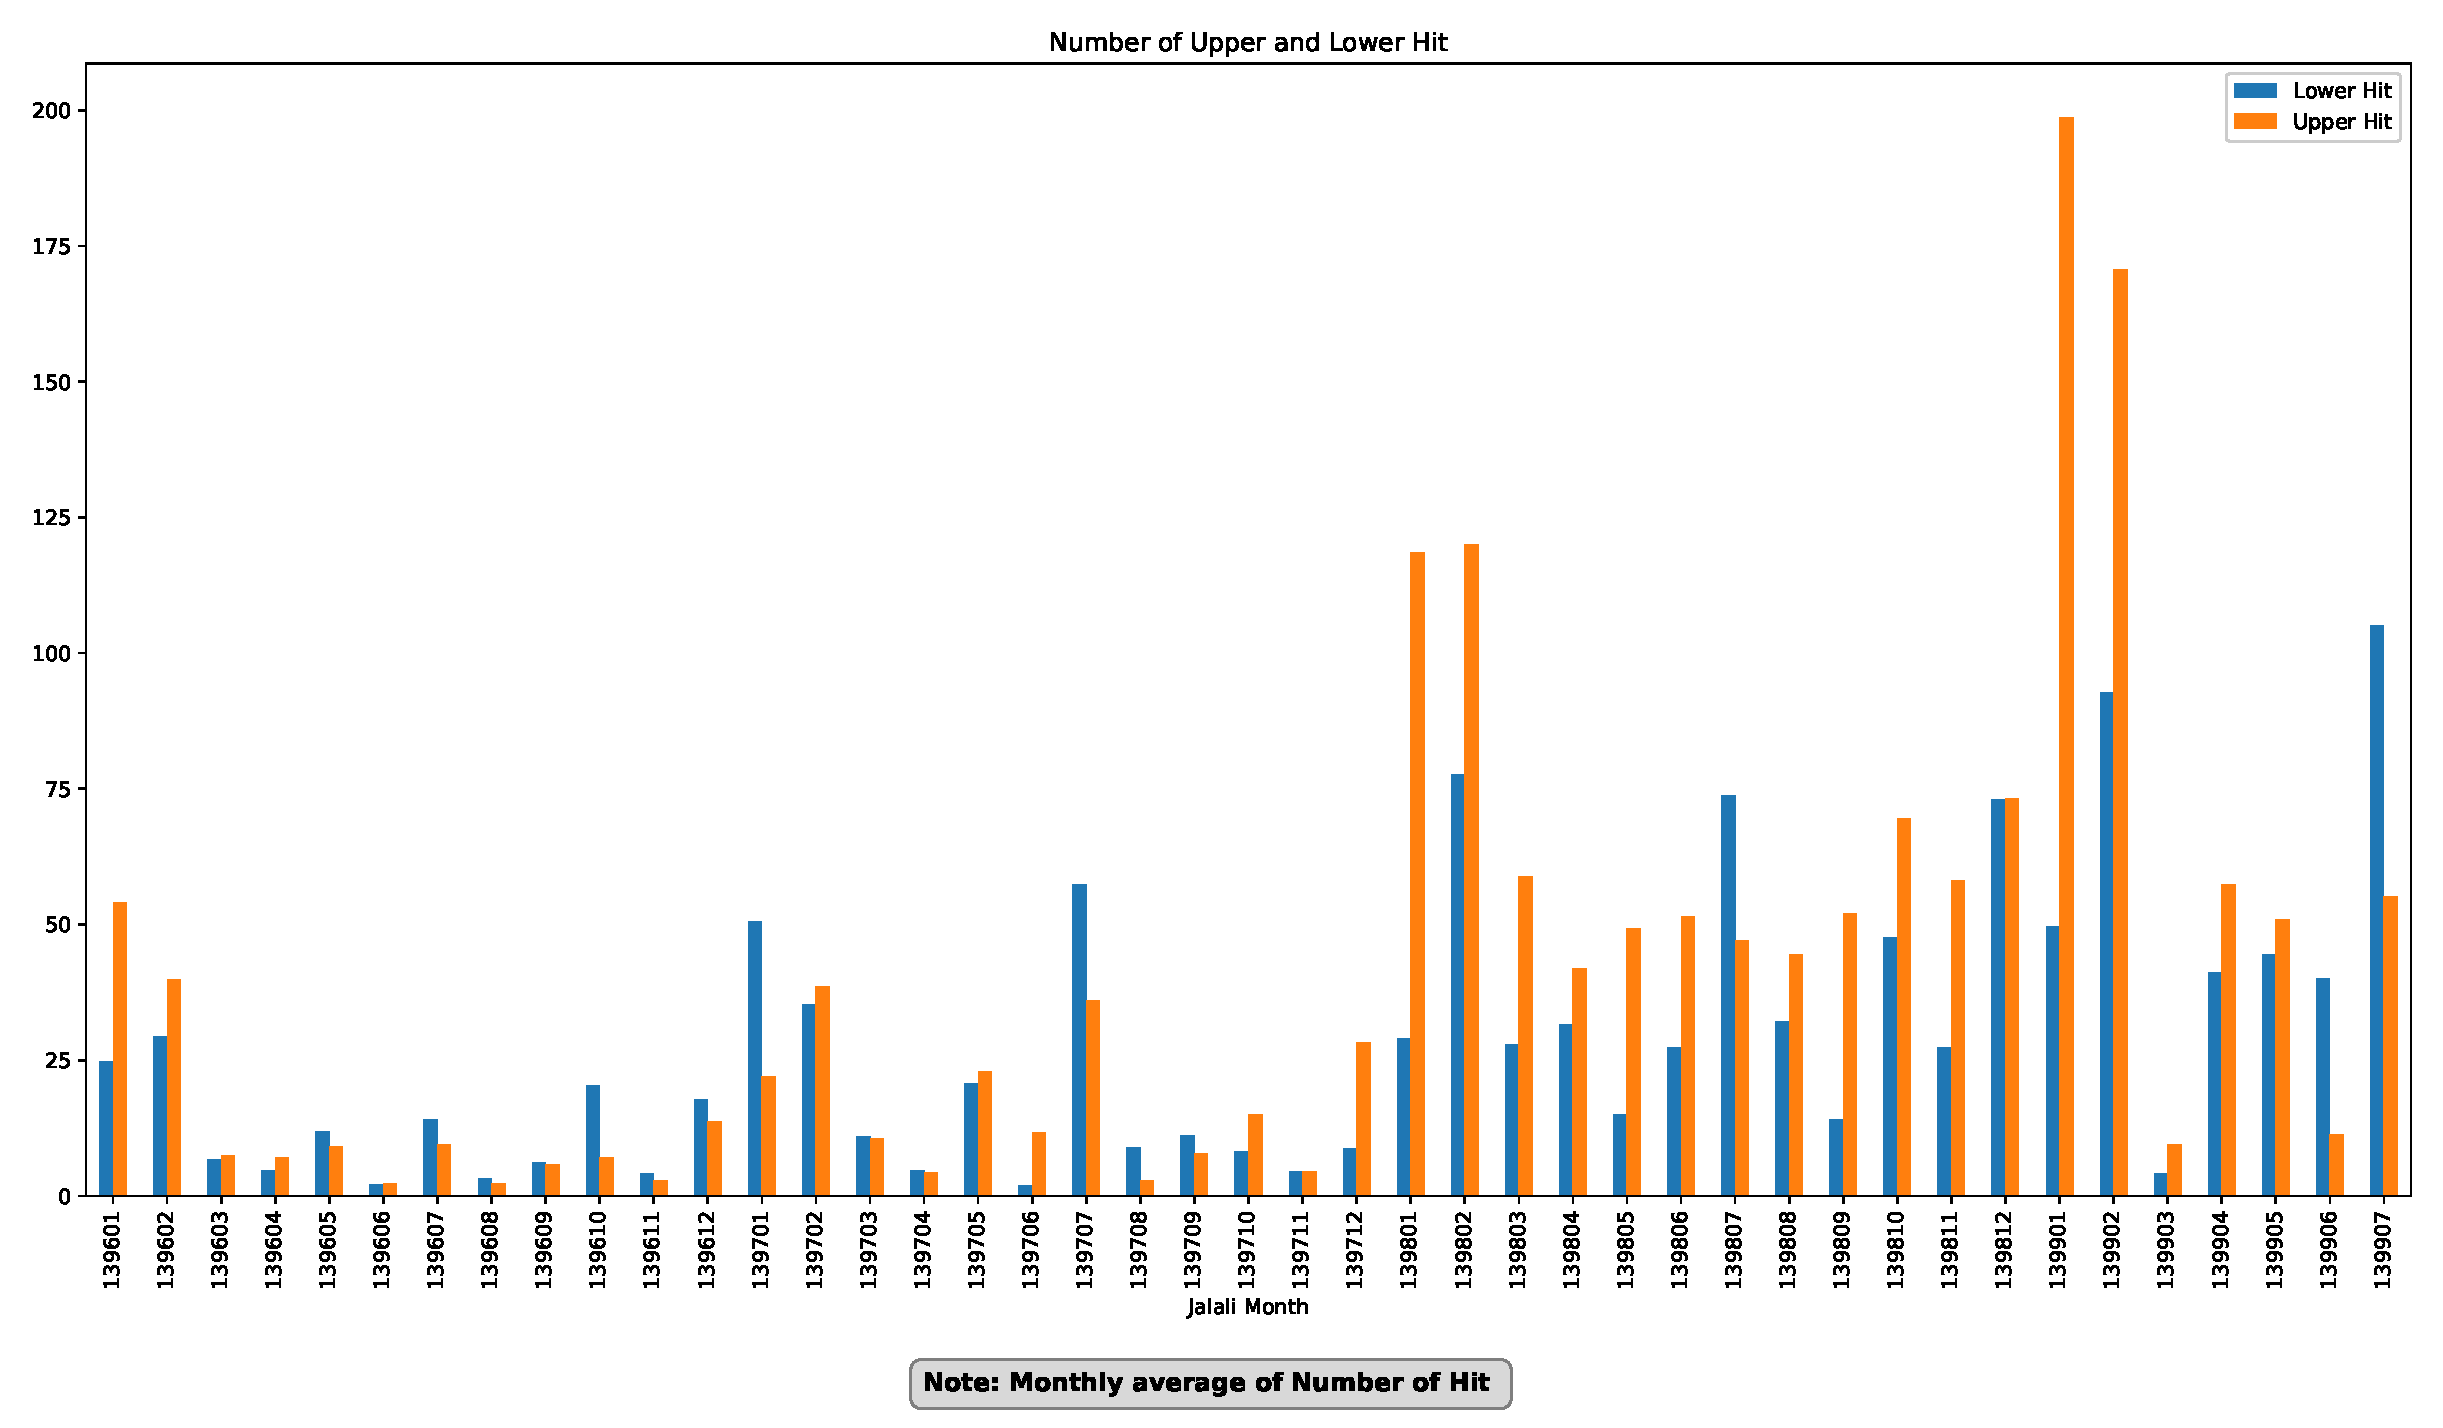
\includegraphics[width=1\linewidth ]{MNH.eps}
\caption{}
\label{fig:mnh}
\end{figure}
\end{landscape}

\begin{landscape}
\begin{figure}
\centering
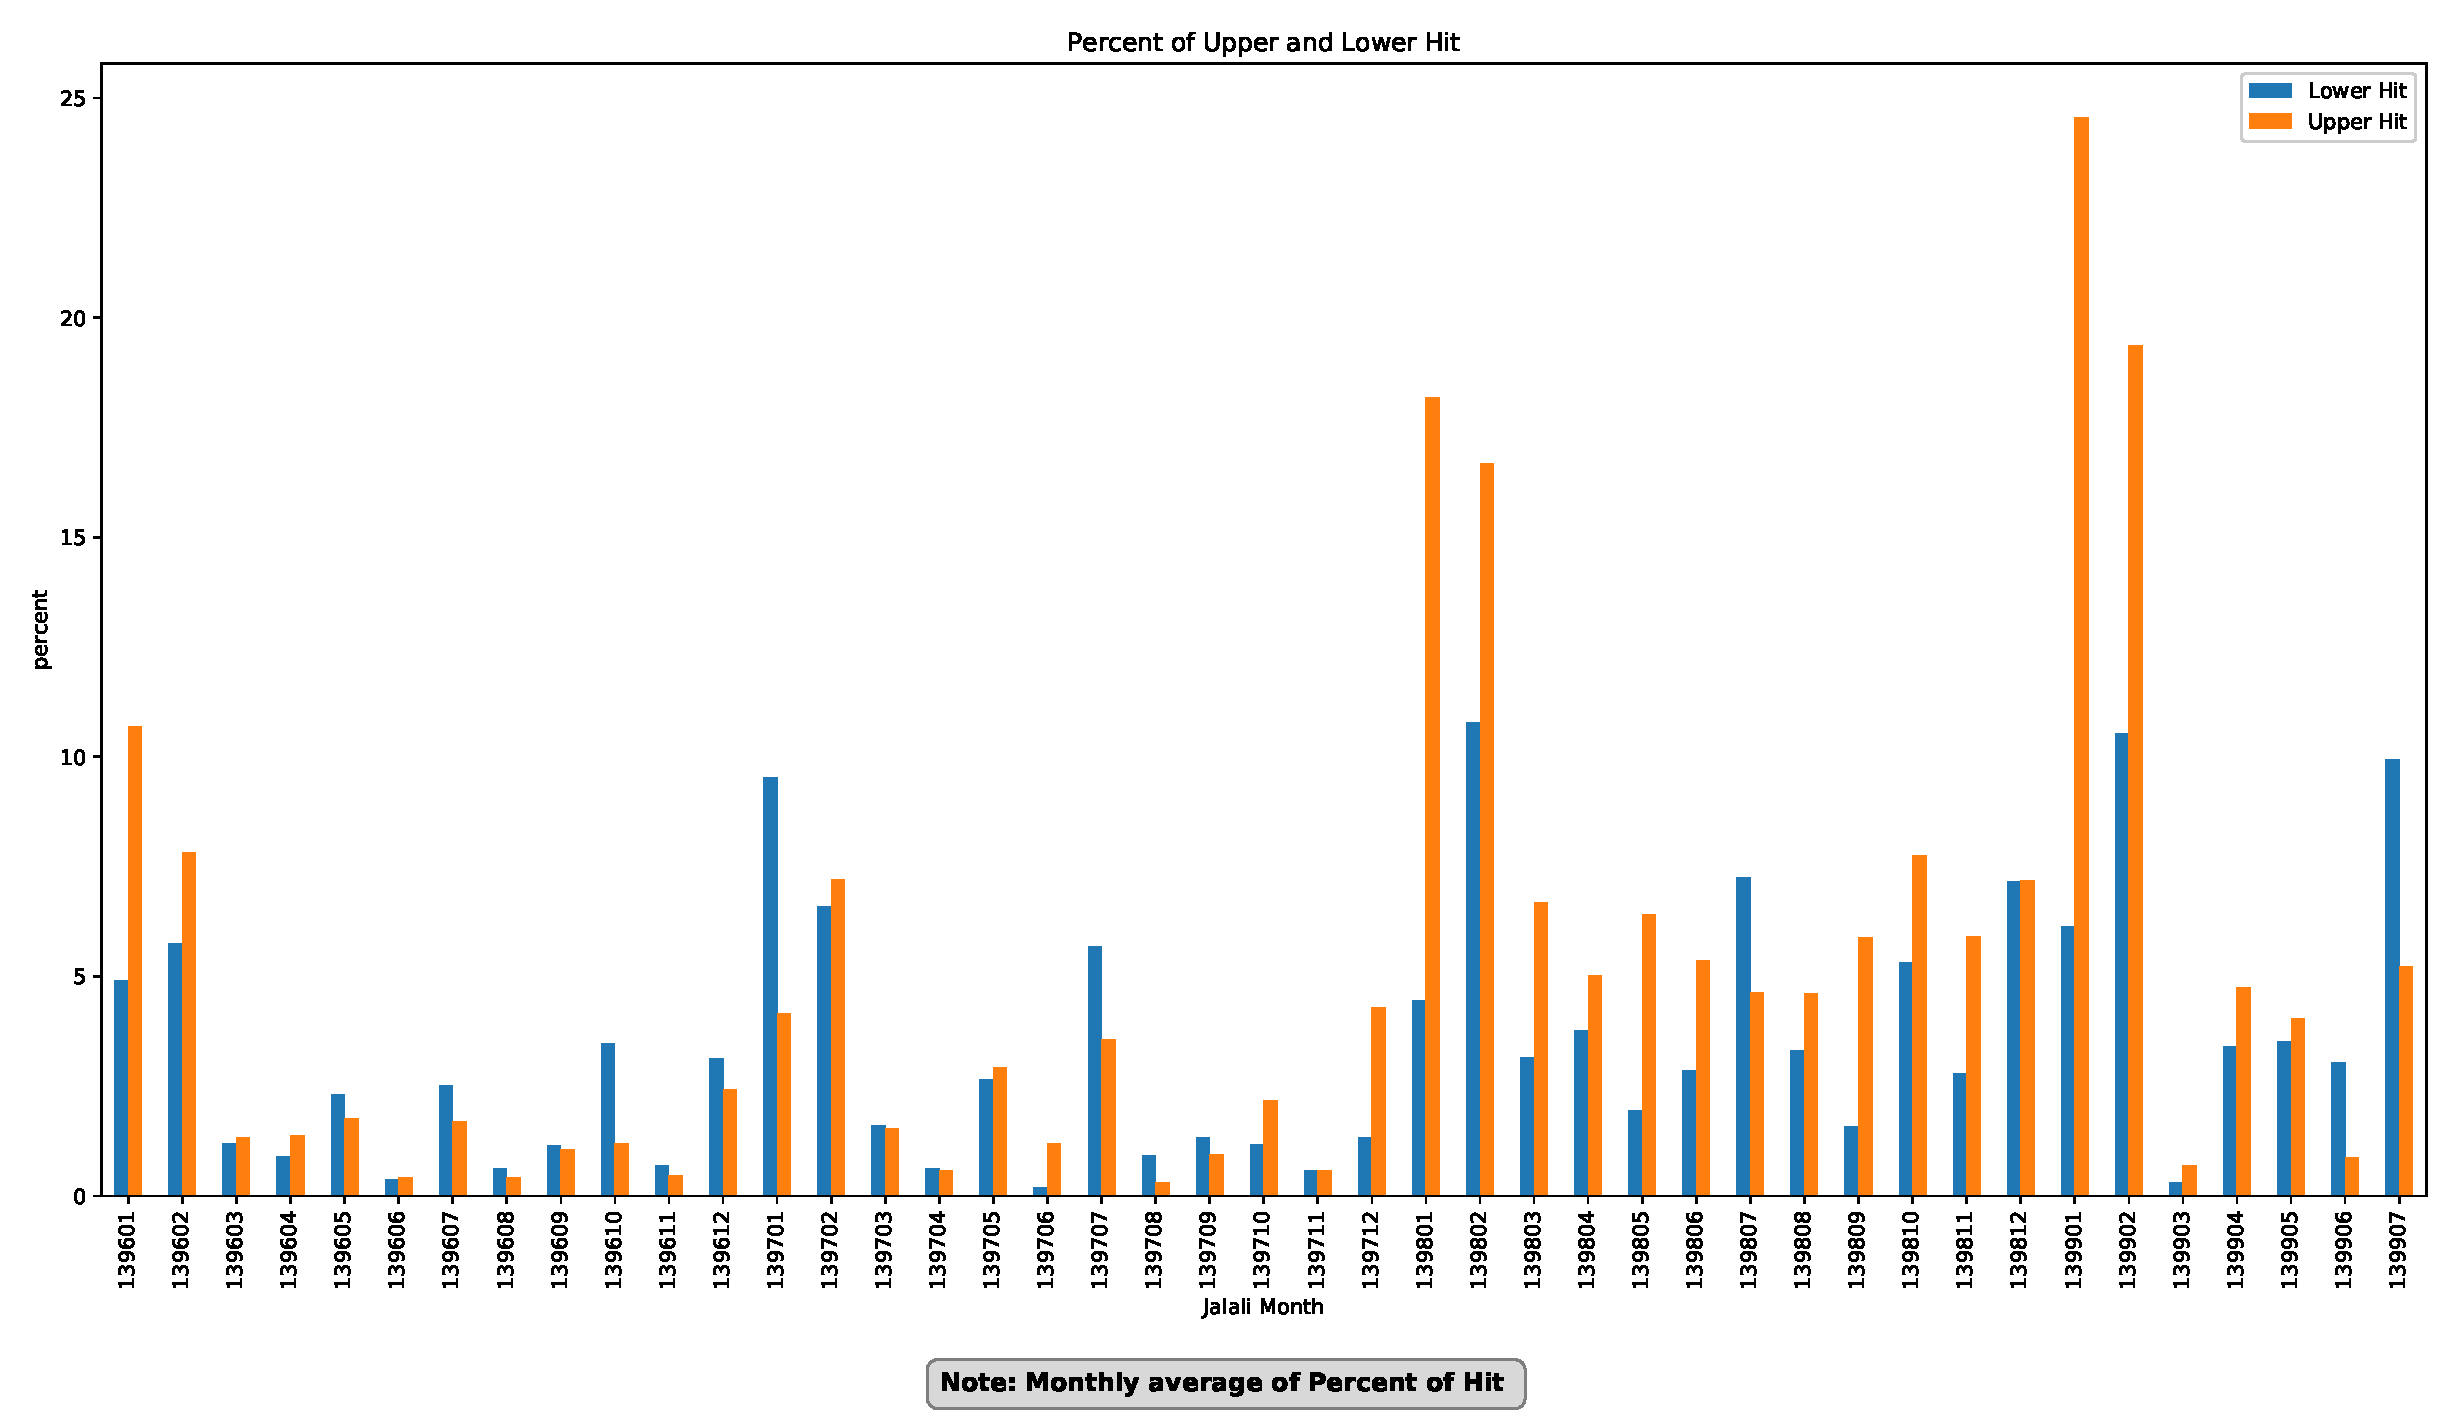
\includegraphics[width=1\linewidth ]{MNH2.eps}
\caption{}
\label{fig:mnh2}
\end{figure}
\end{landscape}



{\begin{table}[htbp]
  \centering
    \begin{tabular}{|l|c|cc|ccccc|}
    \hline
    Event & {count} & {mean} &{std} &{min} & 25\%  & 50\%  & 75\%  & {max} \\
    \hline
        upperHit & 449   & 11.33 & 6.42  & 0     & 7.17  & 10.08 & 13.61 & 50.00 \\
        lowerHit & 449   & 7.88  & 4.24  & 0     & 4.68  & 7.34  & 10.18 & 29.15 \\
        $ u|u $   & 448   & 51.64 & 11.70 & 15.38462 & 44.29 & 51.23 & 58.38 & 94.44 \\
        $ l|u $   & 448   & 12.73 & 6.21  & 0     & 9.32  & 12.44 & 16.00 & 94.44 \\
        $ u|l $   & 447   & 16.96 & 7.72  & 0     & 12.50 & 16.67 & 20.930233 & 91.89 \\
        $ l|l $   & 447   & 37.74 & 10.97 & 0     & 31.0961 & 37.50 & 44.12 & 91.89 \\
        $ u|(u|u) $ & 448   & 7.19  & 5.54  & 0     & 4.09  & 5.89  & 8.71  & 46.72 \\
        $ l|(l|l) $ & 444   & 1.71  & 1.36  & 0     & 0.88  & 1.47  & 2.21  & 12.12 \\
        $ u|(l|l) $ & 448   & 1.77  & 1.28  & 0     & 0.98  & 1.53  & 2.27  & 11.73 \\
        $ l|(u|u) $ & 444   & 3.73  & 2.73  & 0     & 1.83  & 3.25  & 4.86  & 16.95 \\
         \hline
    \end{tabular}
\end{table}}

\begin{figure}[htbp]
\centering
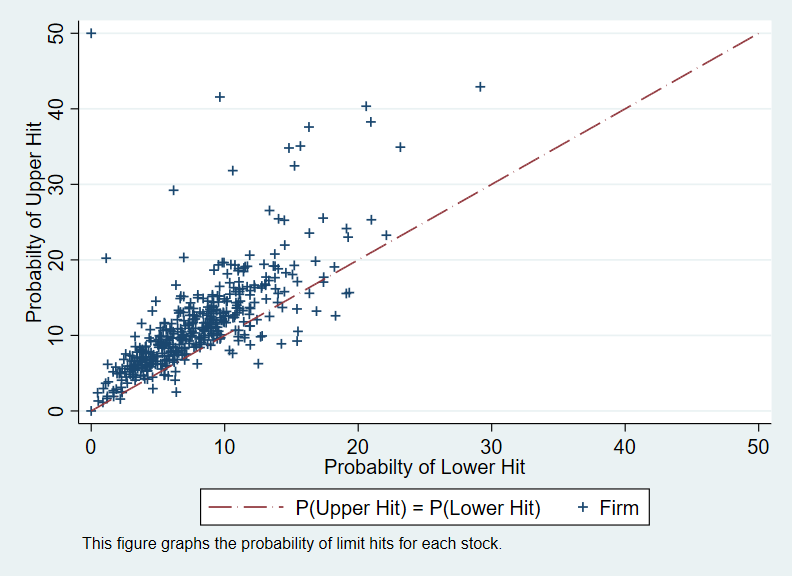
\includegraphics[width=0.65\linewidth]{PUL2.png}
\caption{}
\label{fig:pul2}
\end{figure}
\begin{figure}[htbp]
\centering
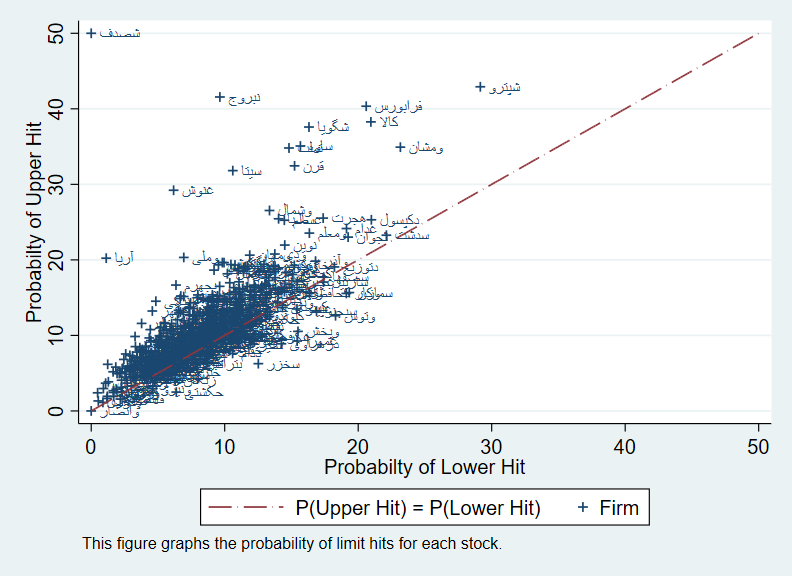
\includegraphics[width=0.65\linewidth]{PUL.png}
\caption{}
\label{fig:pul}
\end{figure}

\begin{figure}[htbp]
\centering
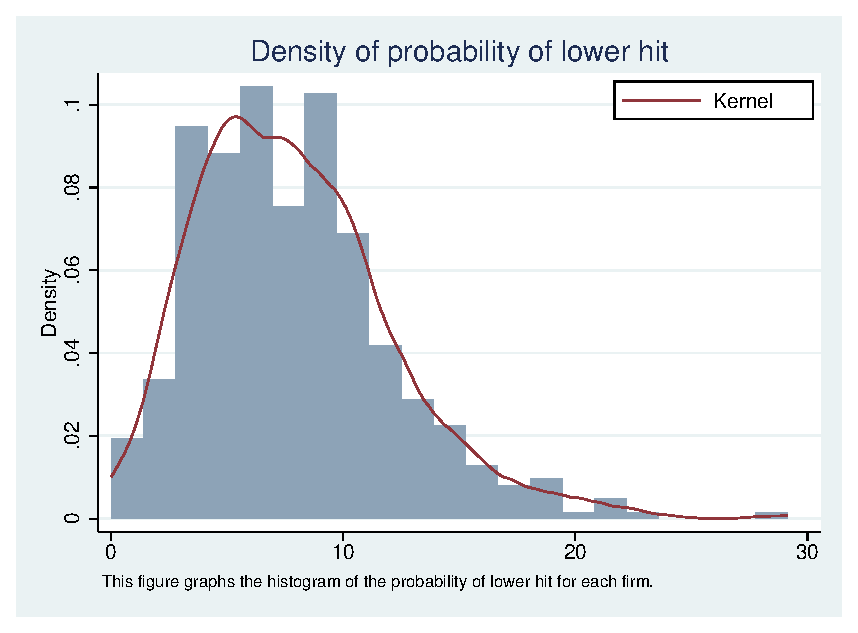
\includegraphics[width=0.7\linewidth]{DPL.eps}
\caption{}
\label{fig:dpl}
\end{figure}
\begin{figure}[htbp]
\centering
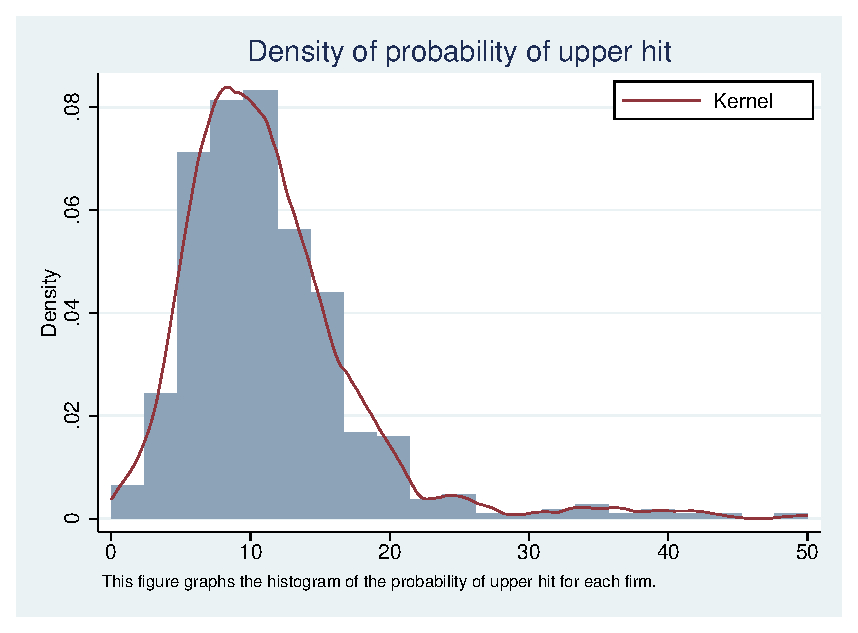
\includegraphics[width=0.7\linewidth]{DPU.eps}
\caption{}
\label{fig:dpu}
\end{figure}

\FloatBarrier
‌ % % % % % % % % % % % % % % %
‌ %  AR 
\section{Abnormal Return}

Abnormal Returns are defined as a difference between the actual return for a stock and the return based on the CAPM equation's 60-day market expectations.
The first step is to calculate the CAPM model coefficients for the asset and then, from that equation, measure the expected return for the asset. 
After that, for calculating abnormal return minus expected return from the actual return of date t+1.

\begin{equation*}
AbR_{t+1} = R_{t+1} - (\hat{\alpha}_{60} + \hat{\beta}_{60} \times (R_{M,t+1}))
\end{equation*}


\begin{figure}[htbp]
\centering
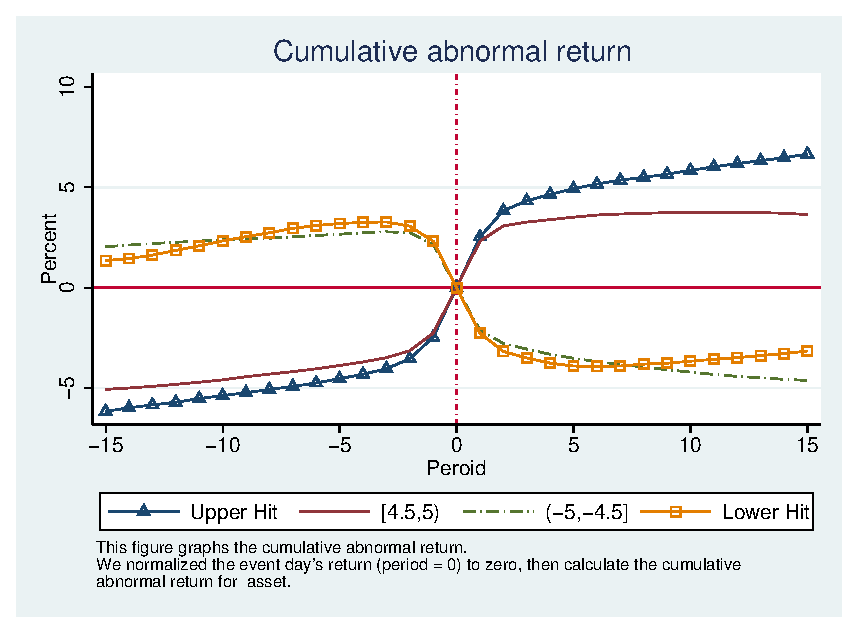
\includegraphics[width=0.7\linewidth]{TAR}
\caption{}
\label{fig:tar}
\end{figure}

\begin{figure}[htbp]
\centering
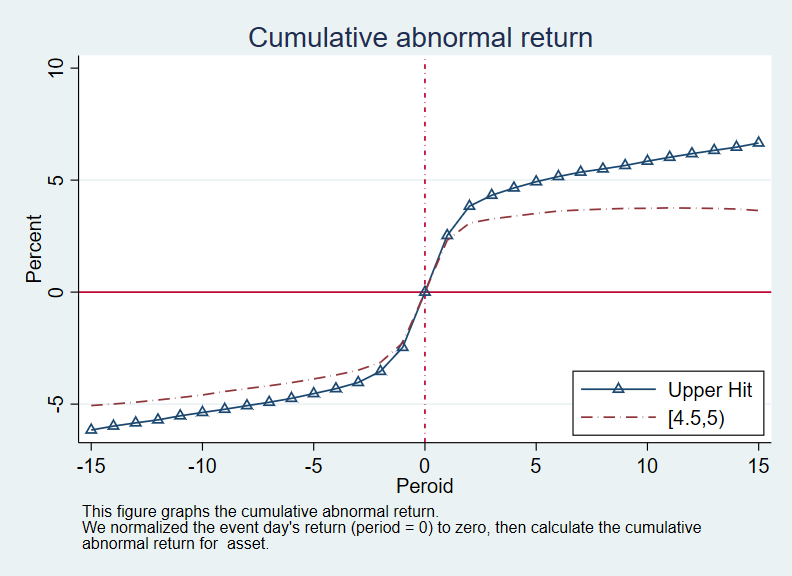
\includegraphics[width=0.7\linewidth]{CUAR}
\caption{}
\label{fig:cuar}
\end{figure}

\begin{figure}[htbp]
\centering
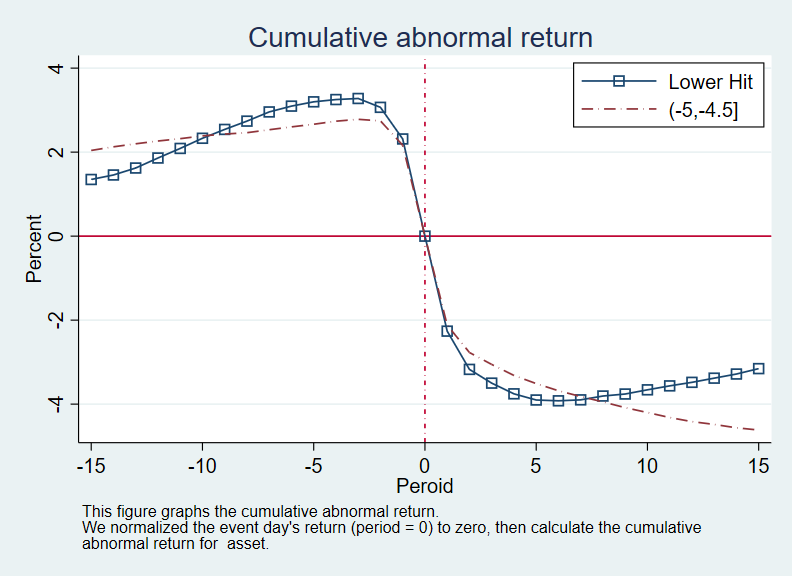
\includegraphics[width=0.7\linewidth]{CLAR}
\caption{}
\label{fig:clar}
\end{figure}

\begin{figure}[htbp]
\centering
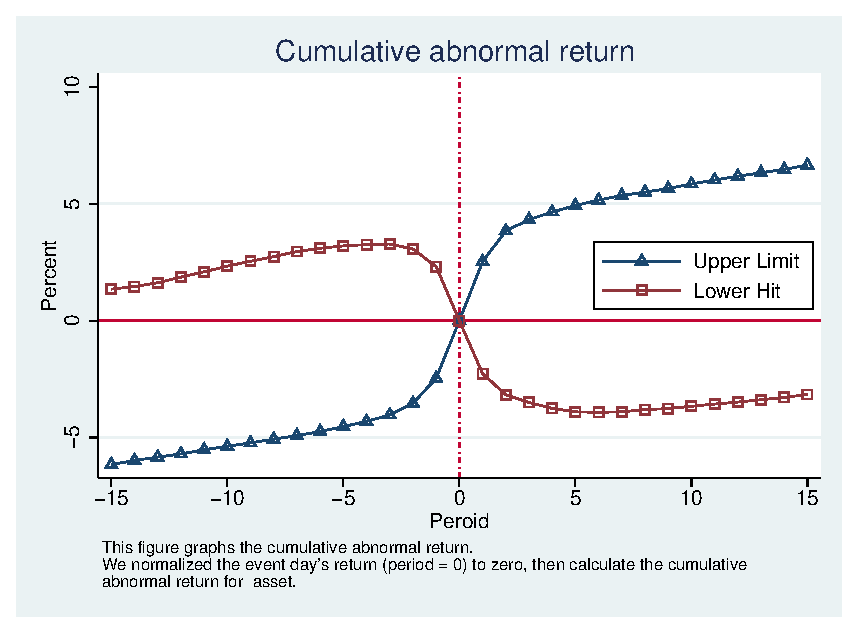
\includegraphics[width=0.7\linewidth]{AR}
\caption{}
\label{fig:ar}
\end{figure}


\begin{figure}[htbp]
\centering
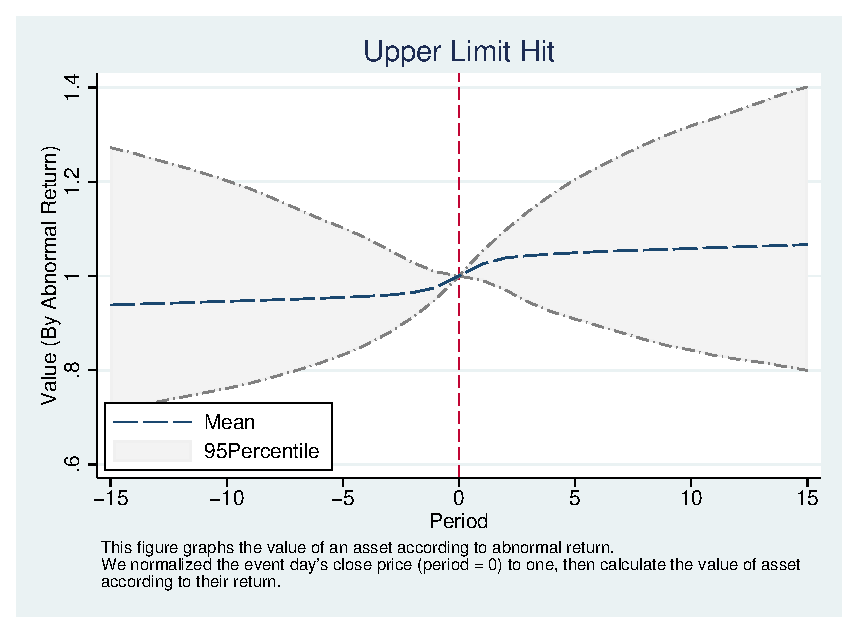
\includegraphics[width=0.7\linewidth]{95U}
\caption{}
\label{fig:95u}
\end{figure}
\begin{figure}[htbp]
\centering
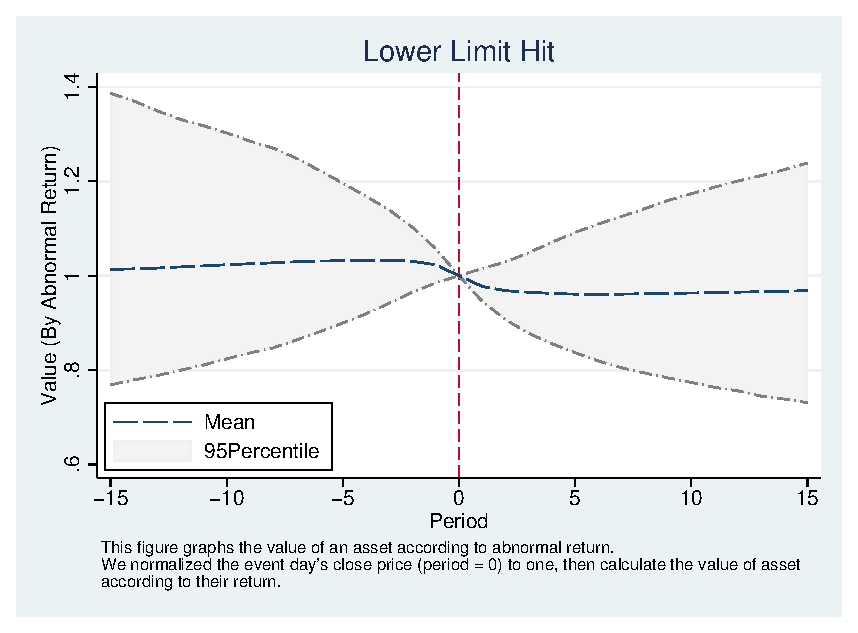
\includegraphics[width=0.7\linewidth]{95L}
\caption{}
\label{fig:95l}
\end{figure}
\begin{figure}[htbp]
\centering
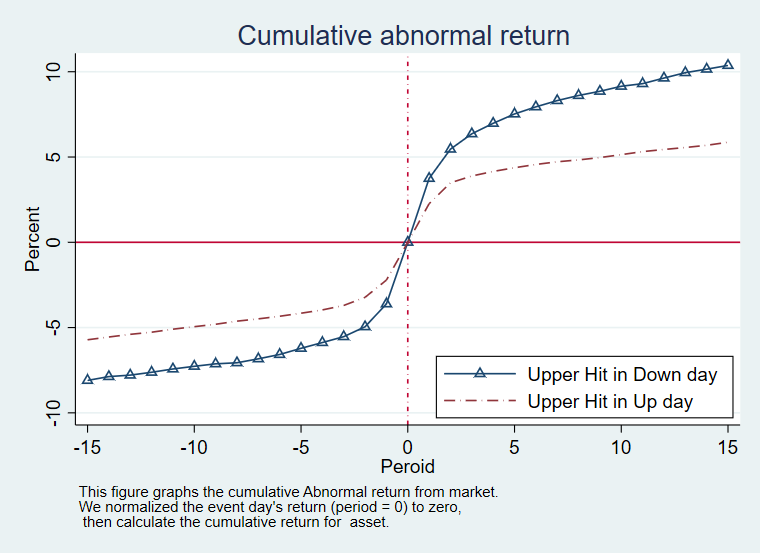
\includegraphics[width=0.7\linewidth]{UPNAbR}
\caption{}
\label{fig:UPNAbR}
\end{figure}
\begin{figure}[htbp]
\centering
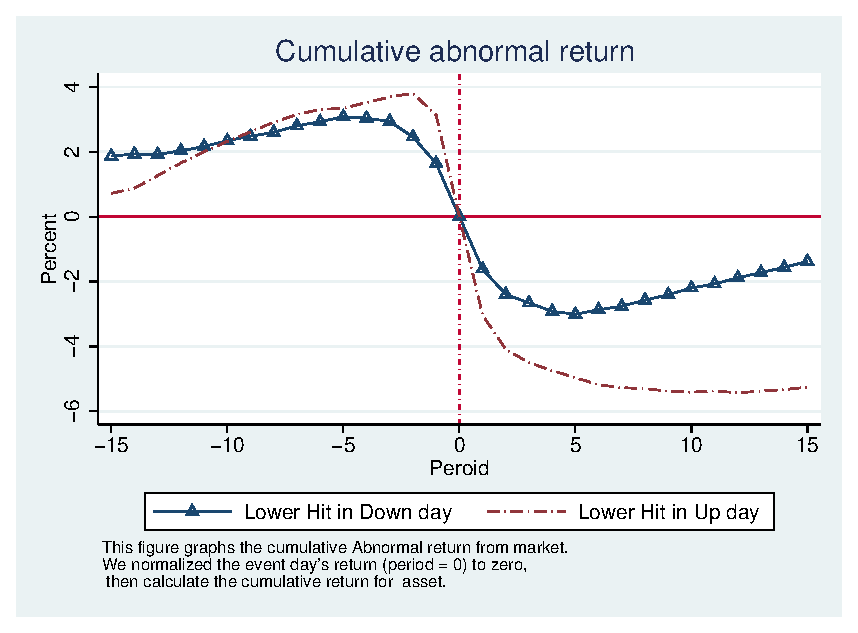
\includegraphics[width=0.7\linewidth]{LPNAbR}
\caption{}
\label{fig:LPNAbR}
\end{figure}
\begin{figure}[htbp]
\centering
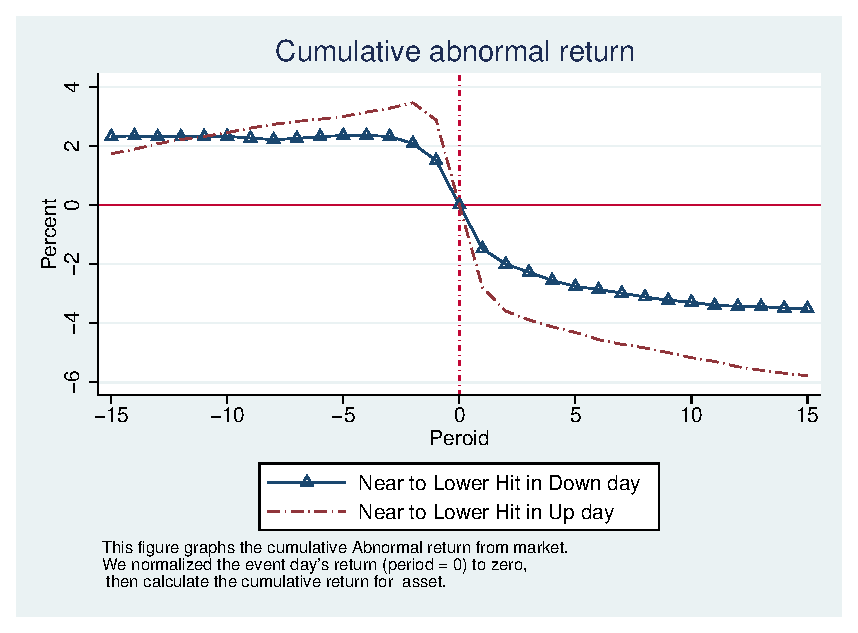
\includegraphics[width=0.7\linewidth]{CLPNAbR}
\caption{}
\label{fig:CLPNAbR}
\end{figure}
\begin{figure}[htbp]
\centering
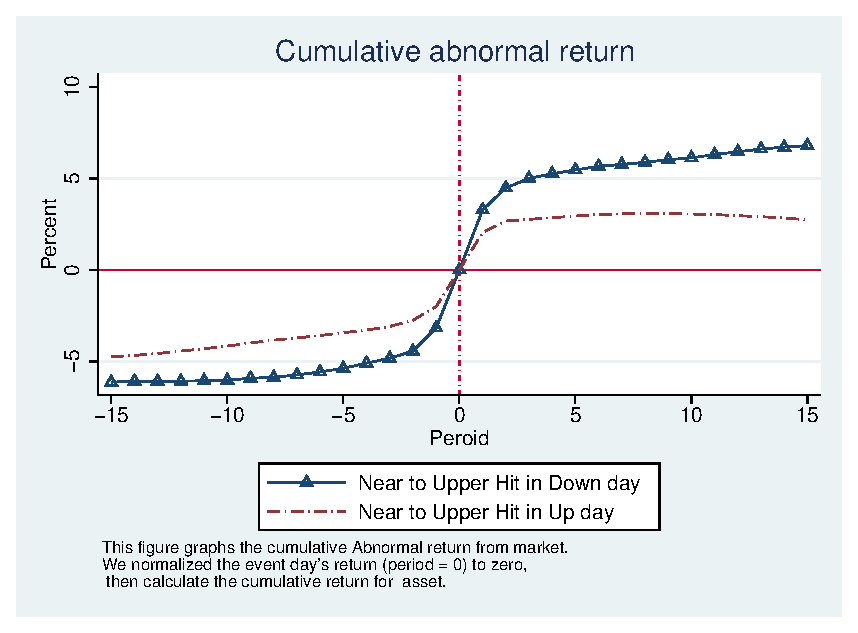
\includegraphics[width=0.7\linewidth]{CUPNAbR}
\caption{}
\label{fig:CUPNAbR}
\end{figure}

\FloatBarrier

\begin{table}[htbp]
\centering

{{
\def\sym#1{\ifmmode^{#1}\else\(^{#1}\)\fi}
\begin{tabular}{l*{6}{c}}
\hline\hline
                    &\multicolumn{1}{c}{(1)}&\multicolumn{1}{c}{(2)}&\multicolumn{1}{c}{(3)}&\multicolumn{1}{c}{(4)}&\multicolumn{1}{c}{(5)}&\multicolumn{1}{c}{(6)}\\
                    &\multicolumn{1}{c}{AbRet\_1}&\multicolumn{1}{c}{AbRet\_2}&\multicolumn{1}{c}{Ab[2,5]}&\multicolumn{1}{c}{Ab[5,50]}&\multicolumn{1}{c}{Ab[50,100]}&\multicolumn{1}{c}{Ab[100,300]}\\
\hline
upperHit            &       3.084\sym{***}&       4.407\sym{***}&       0.766\sym{***}&       19.95\sym{***}&      -4.876\sym{***}&      -19.32\sym{***}\\
                    &     (62.59)         &     (63.66)         &      (9.47)         &     (16.49)         &     (-6.64)         &     (-9.73)         \\
[1em]
[4.5,5)             &       1.630\sym{***}&       2.663\sym{***}&       0.393\sym{***}&      -0.133         &      -1.415\sym{***}&      -1.500         \\
                    &     (71.94)         &     (60.07)         &      (5.25)         &     (-0.18)         &     (-3.40)         &     (-1.66)         \\
[1em]
[4,4.5)             &       0.686\sym{***}&       0.529\sym{***}&      -0.308\sym{***}&       1.697\sym{**} &       0.338         &      -0.831         \\
                    &     (40.16)         &     (15.74)         &     (-4.96)         &      (3.13)         &      (0.97)         &     (-1.02)         \\
[1em]
[2,4)               &       0.641\sym{***}&       0.581\sym{***}&       0.313\sym{***}&       5.033\sym{***}&       0.131         &      -4.315\sym{***}\\
                    &     (26.84)         &     (19.71)         &      (7.71)         &     (12.37)         &      (0.53)         &     (-6.44)         \\
[1em]
(-2,2)              &      -0.211\sym{***}&      -0.423\sym{***}&      0.0324         &      -2.585\sym{***}&      -1.016\sym{*}  &      -1.389         \\
                    &     (-8.38)         &    (-11.43)         &      (0.62)         &     (-4.41)         &     (-2.56)         &     (-1.67)         \\
[1em]
(-4,-2]             &      -1.181\sym{***}&      -1.662\sym{***}&      -0.193\sym{***}&       3.797\sym{***}&      -0.248         &      -3.154\sym{***}\\
                    &    (-58.68)         &    (-54.28)         &     (-4.81)         &      (9.32)         &     (-0.97)         &     (-5.72)         \\
[1em]
(-4.5,-4]           &      -0.599\sym{***}&      -0.686\sym{***}&      -0.134\sym{*}  &       3.222\sym{***}&      -0.262         &      -1.132         \\
                    &    (-33.66)         &    (-20.49)         &     (-2.35)         &      (6.10)         &     (-0.83)         &     (-1.61)         \\
[1em]
(-5,-4.5]           &      -1.161\sym{***}&      -1.614\sym{***}&      -0.820\sym{***}&       1.134         &      -0.599         &       1.716         \\
                    &    (-44.06)         &    (-40.63)         &    (-13.27)         &      (1.74)         &     (-1.49)         &      (1.67)         \\
[1em]
lowerHit            &      -3.049\sym{***}&      -4.350\sym{***}&      -1.344\sym{***}&       12.10\sym{***}&      -1.904\sym{**} &      -3.755\sym{*}  \\
                    &    (-83.61)         &    (-81.26)         &    (-17.95)         &     (10.91)         &     (-3.02)         &     (-2.32)         \\
[1em]
Up Market           &      -1.300\sym{***}&      -1.688\sym{***}&      -0.229\sym{***}&       2.776\sym{***}&      -1.886\sym{***}&      -3.398\sym{***}\\
                    &    (-54.60)         &    (-54.66)         &     (-7.96)         &     (11.47)         &    (-10.50)         &     (-9.23)         \\
[1em]
Constant            &       0.771\sym{***}&       1.257\sym{***}&       0.836\sym{***}&       26.29\sym{***}&       8.578\sym{***}&       29.24\sym{***}\\
                    &     (26.62)         &     (30.04)         &     (10.64)         &     (16.01)         &      (8.77)         &     (15.06)         \\
\hline
Observations        &      305154         &      304705         &      303358         &      282712         &      260818         &      174705         \\
\(R^{2}\)           &       0.428         &       0.327         &       0.011         &       0.033         &       0.008         &       0.029         \\
\hline\hline
\multicolumn{7}{l}{\footnotesize \textit{t} statistics in parentheses}\\
\multicolumn{7}{l}{\footnotesize This table reports fixed effect estimates of abnormal returns. The independent variables are dummies }\\
\multicolumn{7}{l}{\footnotesize  that control for events . We calculate standard errors by using fixed effect on stock level}\\
\multicolumn{7}{l}{\footnotesize \sym{*} \(p<0.05\), \sym{**} \(p<0.01\), \sym{***} \(p<0.001\)}\\
\end{tabular}
}
}
\end{table}

\FloatBarrier

\linespread{0.5}
\section{Trading Strategy}
‌ % % % % % % % % % % % % % % %
‌ % Open close last

\begin{figure}[htbp]
\centering
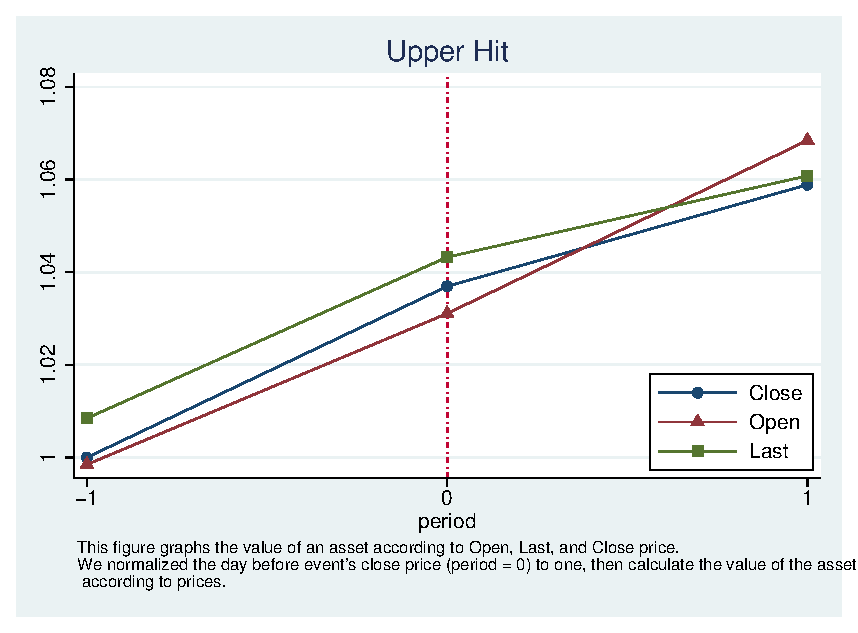
\includegraphics[width=0.6\linewidth]{DUT}
\caption{}
\label{fig:dut}
\end{figure}
\begin{figure}[htbp]
\centering
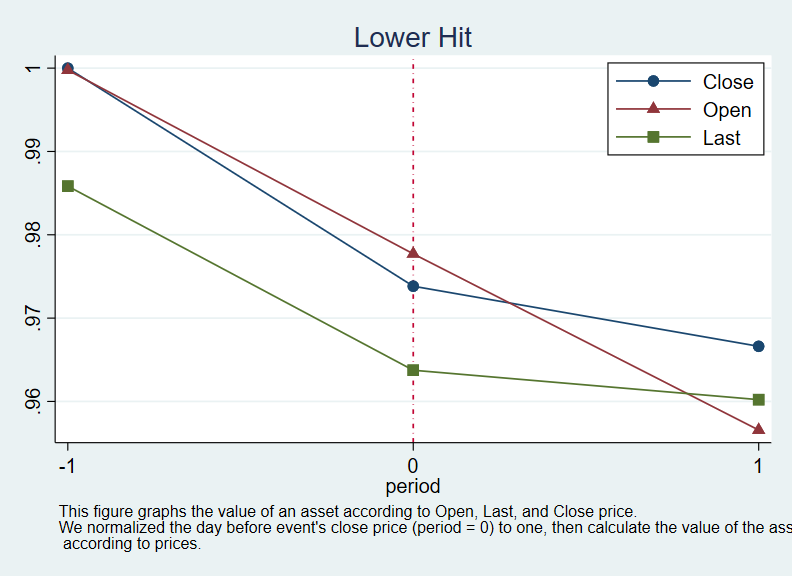
\includegraphics[width=0.65\linewidth]{DLT}
\caption{}
\label{fig:dlt}
\end{figure}

\begin{figure}[htbp]
\centering
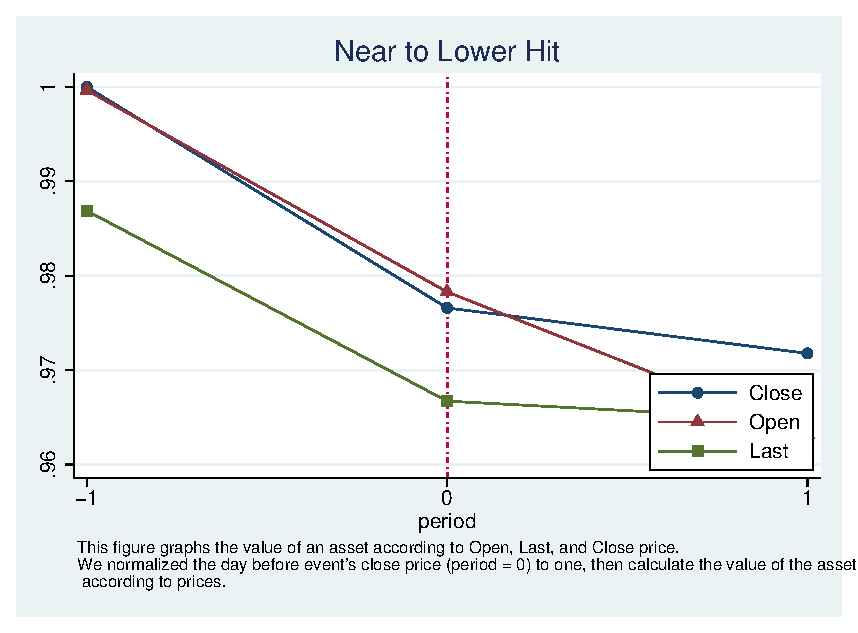
\includegraphics[width=0.7\linewidth]{DCLT}
\caption{}
\label{fig:dclt}
\end{figure}
\begin{figure}[htbp]
\centering
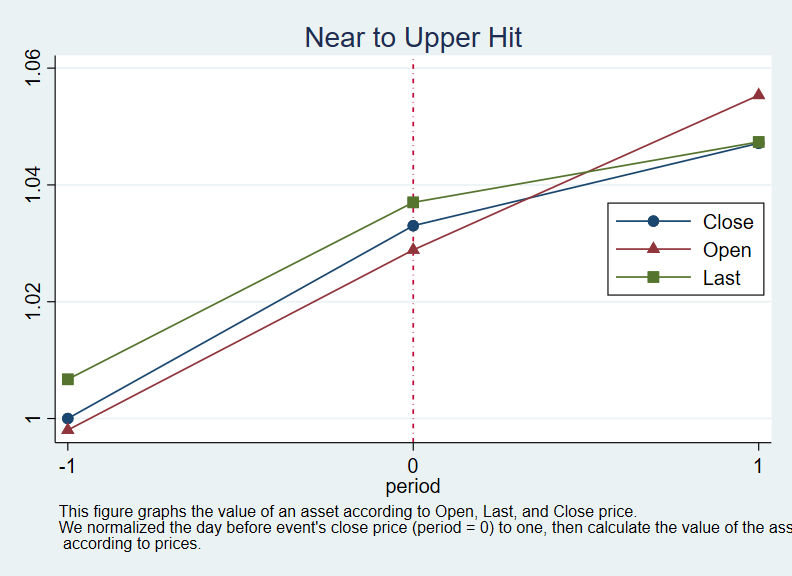
\includegraphics[width=0.7\linewidth]{DCUT}
\caption{}
\label{fig:dcut}
\end{figure}
\FloatBarrier

\linespread{1.5}
\begin{table}[htbp]
\centering

{{
\def\sym#1{\ifmmode^{#1}\else\(^{#1}\)\fi}
\begin{tabular}{l*{6}{c}}
\hline\hline
                    &\multicolumn{1}{c}{(1)}&\multicolumn{1}{c}{(2)}&\multicolumn{1}{c}{(3)}&\multicolumn{1}{c}{(4)}&\multicolumn{1}{c}{(5)}&\multicolumn{1}{c}{(6)}\\
                    &\multicolumn{1}{c}{Close-Open}&\multicolumn{1}{c}{Last-Open}&\multicolumn{1}{c}{TOpen-Last}&\multicolumn{1}{c}{TOpen-Close}&\multicolumn{1}{c}{TOpen-TClose}&\multicolumn{1}{c}{TLast-TOpen}\\
\hline
upperHit            &       0.792\sym{***}&       2.008\sym{***}&       2.587\sym{***}&       3.794\sym{***}&      -1.324\sym{***}&      -0.827\sym{***}\\
                    &      (7.82)         &     (50.88)         &     (68.59)         &     (55.65)         &    (-20.66)         &    (-32.13)         \\
[1em]
[4.5,5)             &       1.070\sym{***}&       1.408\sym{***}&       1.311\sym{***}&       1.662\sym{***}&      -0.270\sym{***}&      -0.222\sym{***}\\
                    &     (26.35)         &     (35.24)         &     (39.27)         &     (43.12)         &     (-8.14)         &     (-6.55)         \\
[1em]
[4,4.5)             &       0.227\sym{***}&       0.293\sym{***}&       0.138\sym{***}&       0.197\sym{***}&      -0.256\sym{***}&      -0.297\sym{***}\\
                    &      (6.57)         &      (7.24)         &      (4.72)         &      (6.31)         &     (-9.08)         &     (-9.25)         \\
[1em]
[2,4)               &      -0.934\sym{***}&      -0.247\sym{***}&       0.503\sym{***}&       1.167\sym{***}&      -0.701\sym{***}&      -0.221\sym{***}\\
                    &    (-14.08)         &     (-9.25)         &     (20.19)         &     (27.68)         &    (-17.79)         &    (-11.50)         \\
[1em]
(-2,2)              &      -0.985\sym{***}&      -0.375\sym{***}&       0.541\sym{***}&       1.133\sym{***}&      -0.505\sym{***}&     -0.0311         \\
                    &    (-15.40)         &    (-15.31)         &     (18.74)         &     (25.99)         &    (-12.70)         &     (-1.33)         \\
[1em]
(-4,-2]             &      -0.786\sym{***}&      -0.730\sym{***}&       0.395\sym{***}&       0.438\sym{***}&      -0.219\sym{***}&     -0.0744\sym{***}\\
                    &    (-23.69)         &    (-34.67)         &     (19.35)         &     (16.22)         &     (-9.22)         &     (-3.80)         \\
[1em]
(-4.5,-4]           &      -0.207\sym{***}&      -0.302\sym{***}&      0.0664\sym{*}  &     -0.0331         &      0.0519         &      0.0645\sym{*}  \\
                    &     (-6.49)         &     (-8.71)         &      (2.35)         &     (-1.04)         &      (1.90)         &      (2.13)         \\
[1em]
(-5,-4.5]           &      -0.505\sym{***}&      -0.530\sym{***}&      -0.192\sym{***}&      -0.198\sym{***}&       0.291\sym{***}&       0.241\sym{***}\\
                    &    (-12.18)         &    (-15.32)         &     (-5.98)         &     (-5.05)         &      (8.90)         &      (7.63)         \\
[1em]
lowerHit            &      -1.452\sym{***}&      -1.813\sym{***}&      -0.631\sym{***}&      -0.987\sym{***}&       0.464\sym{***}&       0.337\sym{***}\\
                    &    (-28.53)         &    (-47.08)         &    (-19.17)         &    (-27.25)         &     (13.36)         &     (10.44)         \\
[1em]
Constant            &       0.734\sym{***}&       0.107\sym{***}&      -0.402\sym{***}&      -1.012\sym{***}&       0.581\sym{***}&       0.157\sym{***}\\
                    &     (12.22)         &      (3.89)         &    (-13.26)         &    (-21.91)         &     (14.34)         &      (6.00)         \\
\hline
Observations        &      245107         &      245107         &      245105         &      245105         &      245103         &      245103         \\
\(R^{2}\)           &       0.083         &       0.138         &       0.102         &       0.176         &       0.048         &       0.016         \\
\hline\hline
\multicolumn{7}{l}{\footnotesize \textit{t} statistics in parentheses}\\
\multicolumn{7}{l}{\footnotesize \sym{*} \(p<0.05\), \sym{**} \(p<0.01\), \sym{***} \(p<0.001\)}\\
\end{tabular}
}
}
\end{table}

\FloatBarrier

‌ % % % % % % % % % % % % % % %
‌ % I

\section{Buy-Sell Imbalances}
Buy-sell imbalances for each type is defined as the net buying ratio of stock k on date t by a particular type to the amounts bought and sold by that type.

\begin{equation*}
\begin{matrix}
\text{Imbalance}_{k,t}^{\text{Indiv}} = \frac{\text{Buys}_{k,t}^{\text{Indiv}} - \text{Sells}_{k,t}^{\text{Indiv}}}{\text{Buys}_{k,t}^{\text{Indiv}} + \text{Sells}_{k,t}^{\text{Indiv}}} & & &  \text{Imbalance}_{k,t}^{\text{Inst}} = \frac{\text{Buys}_{k,t}^{\text{Inst}} - \text{Sells}_{k,t}^{\text{Inst}}}{\text{Buys}_{k,t}^{\text{Inst}} + \text{Sells}_{k,t}^{\text{Inst}}}
\end{matrix}
\end{equation*}


\begin{figure}[htbp]
\centering
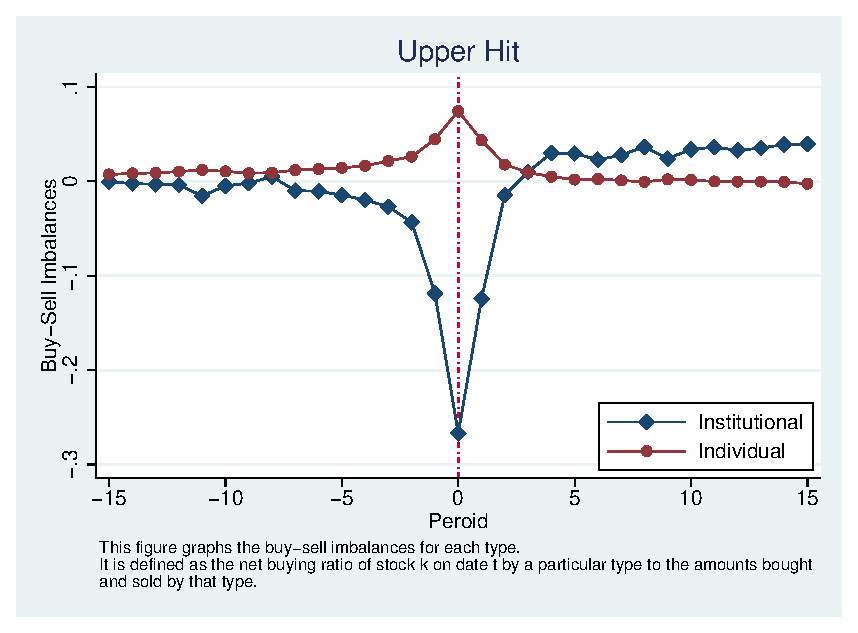
\includegraphics[width=0.7\linewidth]{UI}
\caption{}
\label{fig:ui}
\end{figure}

\begin{figure}[htbp]
\centering
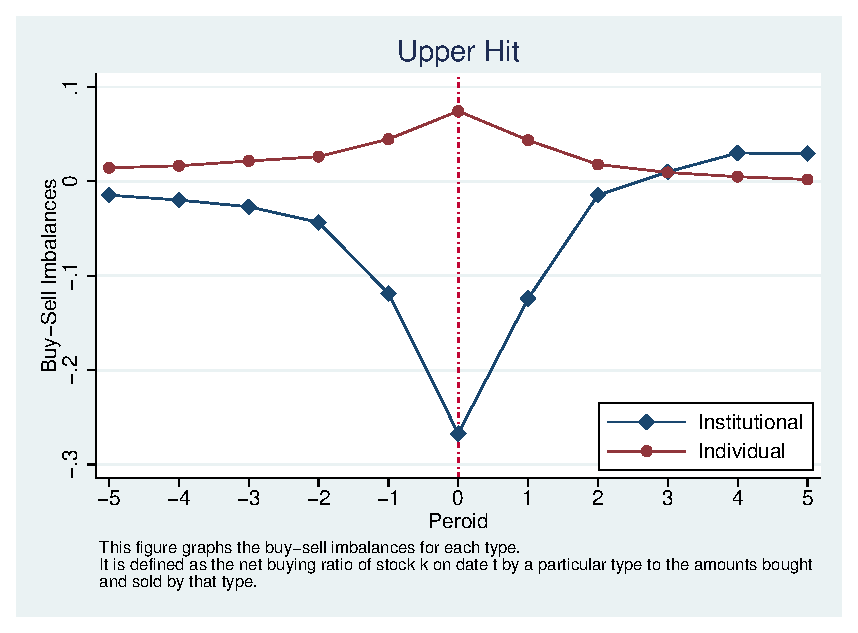
\includegraphics[width=0.7\linewidth]{UI2.eps}
\caption{}
\label{fig:ui2}
\end{figure}

\begin{figure}[htbp]
\centering
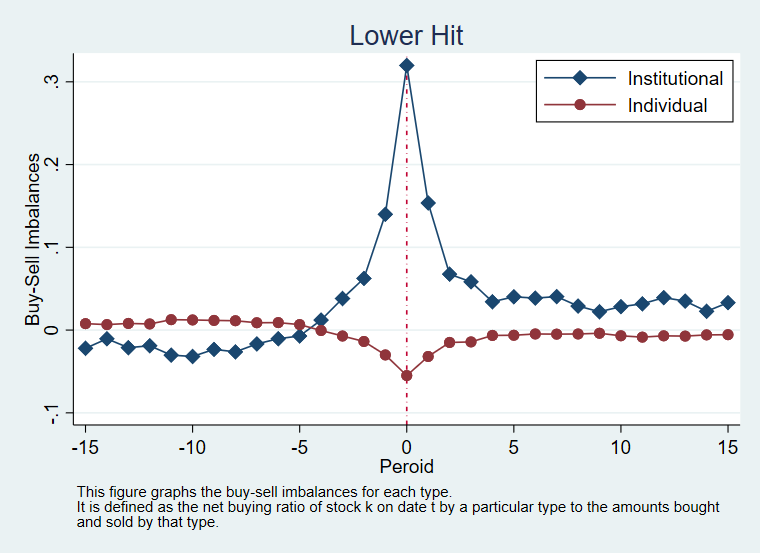
\includegraphics[width=0.7\linewidth]{LI}
\caption{}
\label{fig:li}
\end{figure}
\begin{figure}[htbp]
\centering
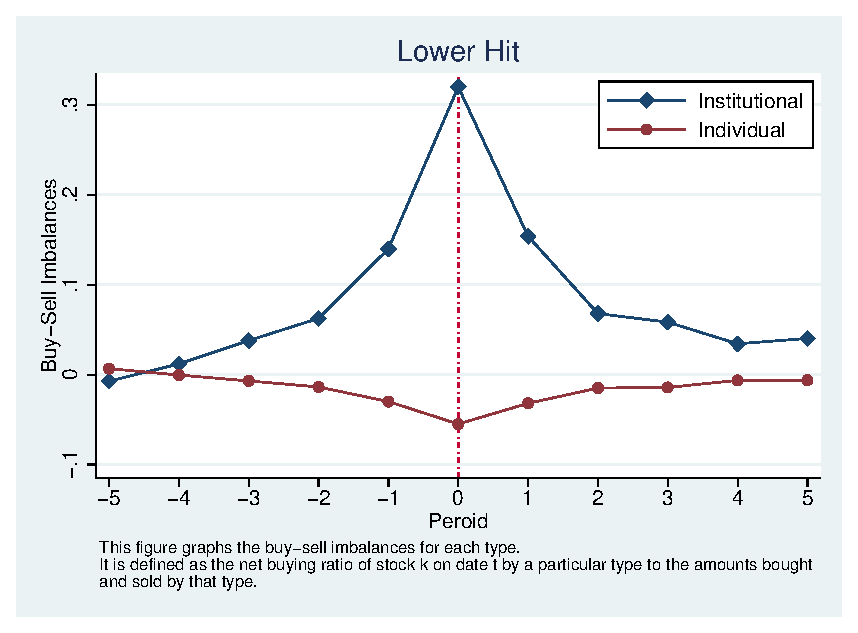
\includegraphics[width=0.7\linewidth]{LI2.eps}
\caption{}
\label{fig:li2}
\end{figure}


\begin{figure}[htbp]
\centering
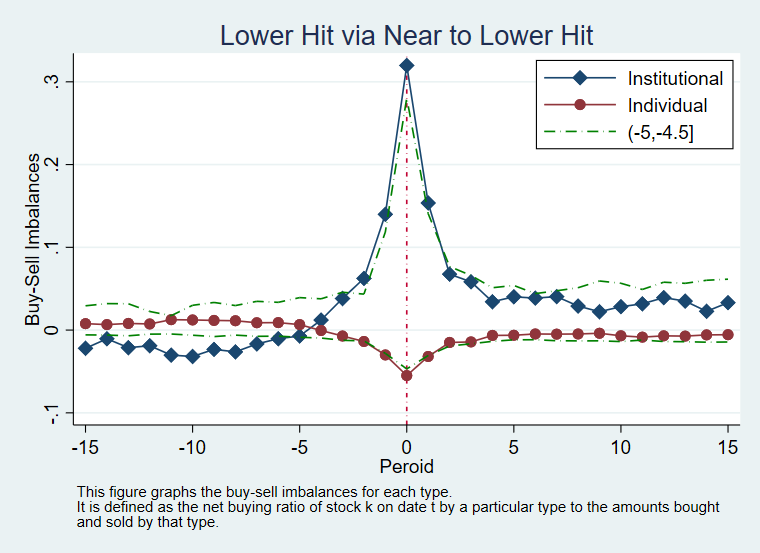
\includegraphics[width=0.7\linewidth]{CLI}
\caption{}
\label{fig:cli}
\end{figure}



\begin{figure}[htbp]
\centering
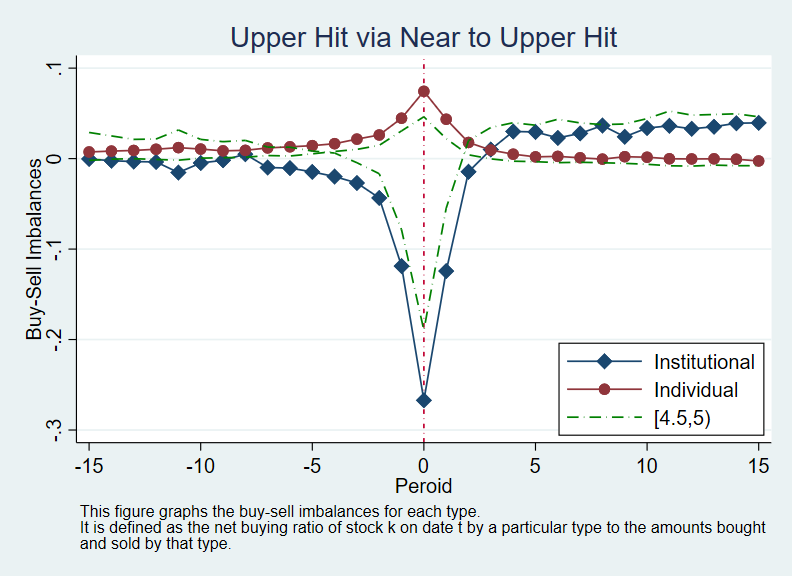
\includegraphics[width=0.7\linewidth]{TUI}
\caption{}
\label{fig:tui}
\end{figure}

\begin{figure}[htbp]
\centering
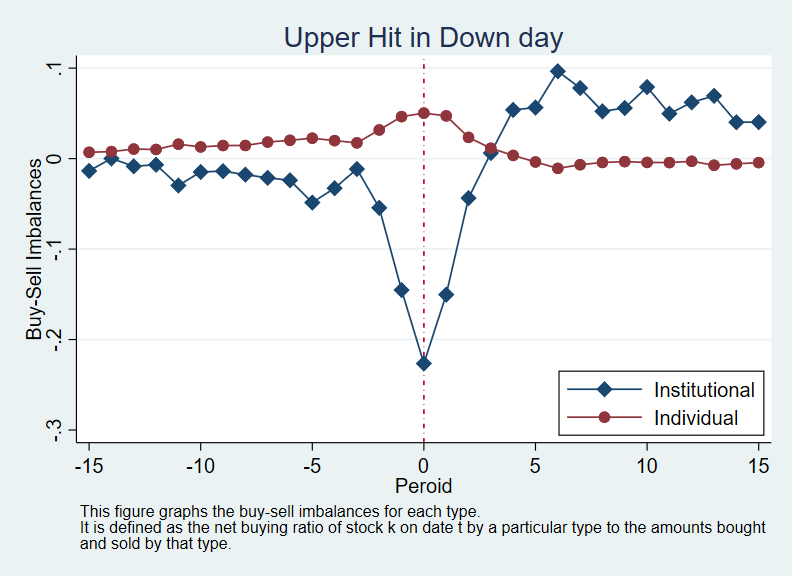
\includegraphics[width=0.7\linewidth]{NUI}
\caption{}
\label{fig:NUI}
\end{figure}


\begin{figure}[htbp]
\centering
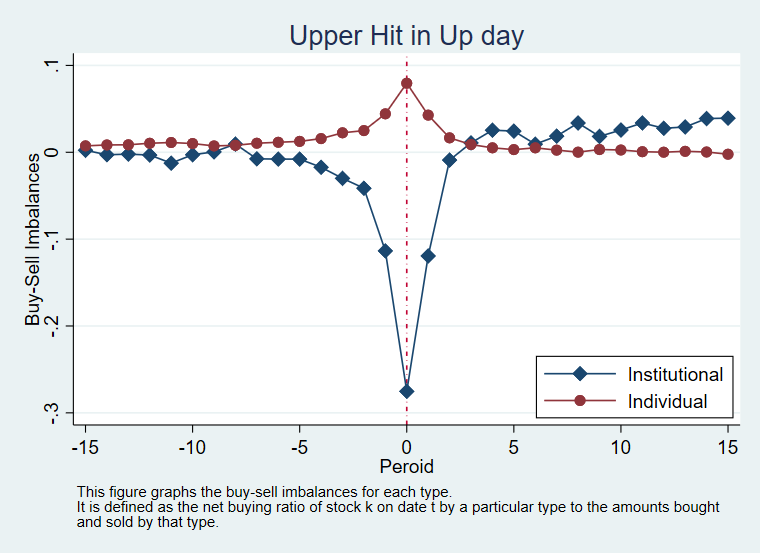
\includegraphics[width=0.7\linewidth]{PUI}
\caption{}
\label{fig:PUI}
\end{figure}


\begin{figure}[htbp]
\centering
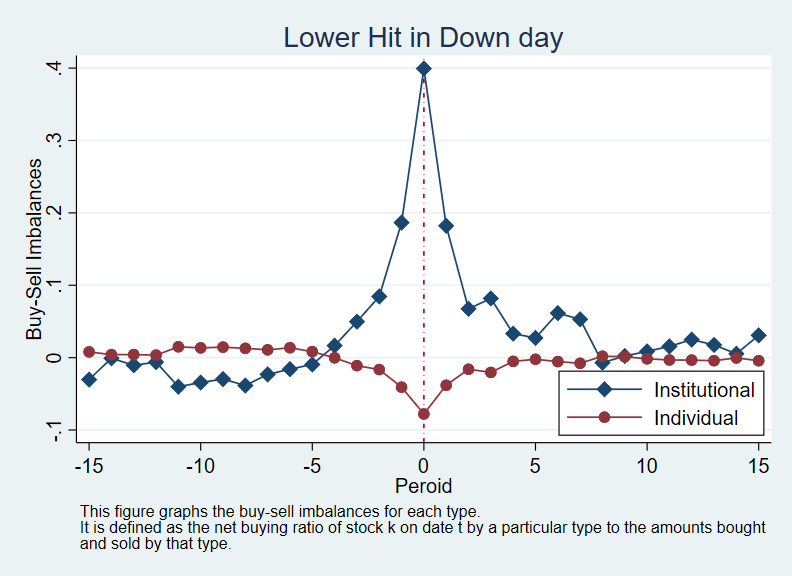
\includegraphics[width=0.7\linewidth]{NLI}
\caption{}
\label{fig:NLI}
\end{figure}


\begin{figure}[htbp]
\centering
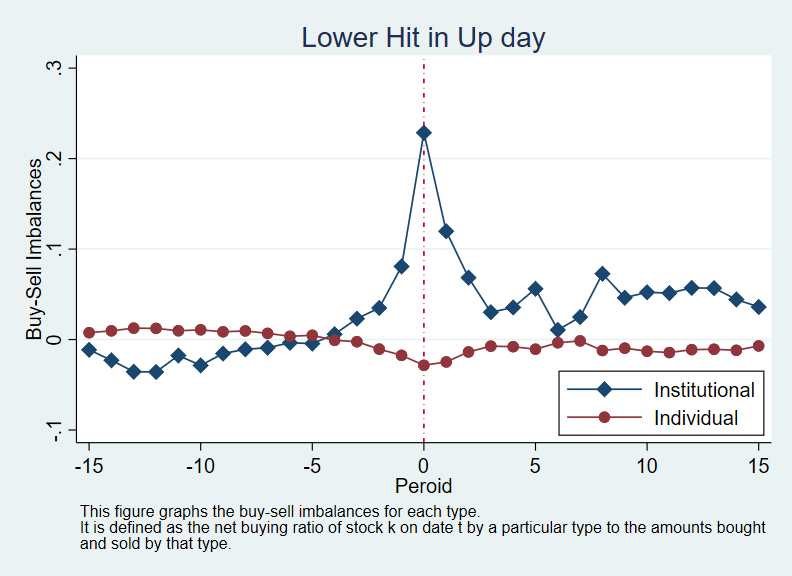
\includegraphics[width=0.7\linewidth]{PLI}
\caption{}
\label{fig:PLI}
\end{figure}


\FloatBarrier

\begin{table}[htbp]
\centering

{{
\def\sym#1{\ifmmode^{#1}\else\(^{#1}\)\fi}
\begin{tabular}{l*{4}{c}}
\hline\hline
                    &\multicolumn{1}{c}{(1)}&\multicolumn{1}{c}{(2)}&\multicolumn{1}{c}{(3)}&\multicolumn{1}{c}{(4)}\\
                    &\multicolumn{1}{c}{InslImbalance}&\multicolumn{1}{c}{FInslImbalance}&\multicolumn{1}{c}{IndlImbalance}&\multicolumn{1}{c}{FIndlImbalance}\\
\hline
upperHit            &      -0.603\sym{***}&      -0.325\sym{***}&       0.141\sym{***}&      0.0910\sym{***}\\
                    &    (-38.54)         &    (-24.89)         &     (21.03)         &     (16.91)         \\
[1em]
[4.5,5)             &      -0.256\sym{***}&      -0.160\sym{***}&      0.0697\sym{***}&      0.0403\sym{***}\\
                    &    (-22.62)         &    (-13.71)         &     (19.08)         &     (13.32)         \\
[1em]
[4,4.5)             &     -0.0778\sym{***}&     -0.0128         &      0.0117\sym{***}&     0.00778\sym{**} \\
                    &     (-7.76)         &     (-1.21)         &      (4.85)         &      (2.98)         \\
[1em]
[2,4)               &      -0.169\sym{***}&     -0.0770\sym{***}&      0.0280\sym{***}&      0.0216\sym{***}\\
                    &    (-23.23)         &    (-10.62)         &     (10.07)         &      (9.09)         \\
[1em]
(-2,2)              &     -0.0540\sym{***}&     -0.0383\sym{***}&     -0.0189\sym{***}&     -0.0110\sym{*}  \\
                    &     (-5.06)         &     (-3.81)         &     (-3.51)         &     (-2.24)         \\
[1em]
(-4,-2]             &    -0.00104         &     -0.0260\sym{***}&   -0.000676         &     0.00323         \\
                    &     (-0.17)         &     (-4.40)         &     (-0.30)         &      (1.66)         \\
[1em]
(-4.5,-4]           &      0.0120         &     -0.0157         &     0.00840\sym{***}&     0.00590\sym{*}  \\
                    &      (1.29)         &     (-1.52)         &      (3.66)         &      (2.19)         \\
[1em]
(-5,-4.5]           &     -0.0152         &     -0.0357\sym{***}&      0.0166\sym{***}&      0.0145\sym{***}\\
                    &     (-1.46)         &     (-3.38)         &      (6.08)         &      (4.98)         \\
[1em]
lowerHit            &       0.110\sym{***}&     -0.0239\sym{*}  &     0.00298         &      0.0173\sym{***}\\
                    &      (8.38)         &     (-2.00)         &      (0.64)         &      (3.99)         \\
[1em]
Constant            &       0.314\sym{***}&       0.227\sym{***}&     -0.0699\sym{***}&     -0.0564\sym{***}\\
                    &     (24.73)         &     (17.17)         &     (-9.91)         &     (-7.85)         \\
\hline
Observations        &      176979         &      176740         &      245076         &      244653         \\
\(R^{2}\)           &       0.083         &       0.021         &       0.046         &       0.020         \\
\hline\hline
\multicolumn{5}{l}{\footnotesize \textit{t} statistics in parentheses}\\
\multicolumn{5}{l}{\footnotesize \sym{*} \(p<0.05\), \sym{**} \(p<0.01\), \sym{***} \(p<0.001\)}\\
\end{tabular}
}
}
\end{table}


\FloatBarrier

‌ % % % % % % % % % % % % % % %
‌ % T
\section{Volume}
Turnover of stock is defined as the amount traded in Rial divided by the stock's market capitalization. Based on this factor, we define Relative Turnover by the ratio of the turnover of stock k on date t to the 60 days average turnover of stock k.
\begin{equation*}
\begin{matrix}
\text{Turn}_{k,t} = \frac{\text{Volume}(\text{Rial})_{k,t}}{\text{MarketCap}_{k,t}}&&&&
\text{RelTurn}_{k,t} = \frac{\text{Turn}_{k,t}}{AVG_{60}(\text{Turn}_{k,t})}
\end{matrix}
\end{equation*}

\subsection{Turnover}

\begin{figure}[htbp]
\centering
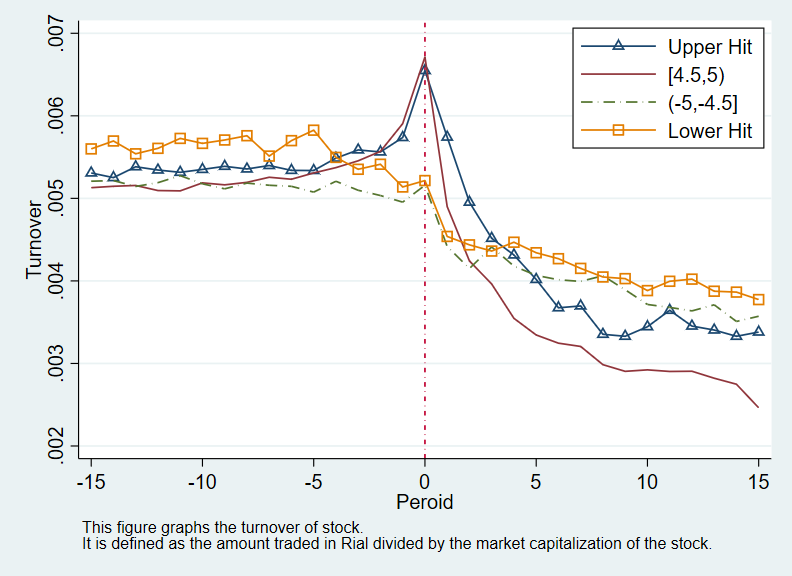
\includegraphics[width=0.7\linewidth]{TT}
\caption{}
\label{fig:tt}
\end{figure}

\begin{figure}[htbp]
\centering
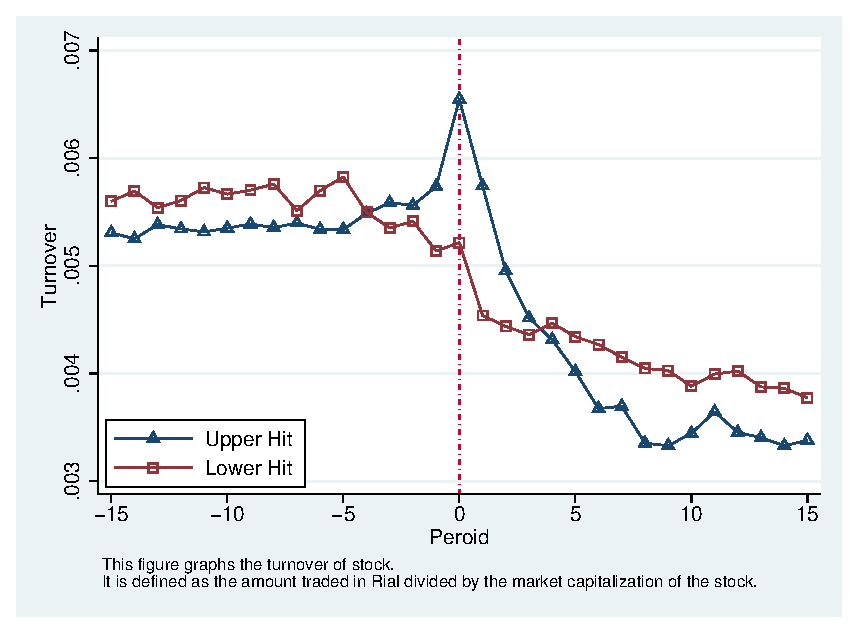
\includegraphics[width=0.7\linewidth]{T}
\caption{}
\label{fig:t}
\end{figure}

\begin{figure}[htbp]
\centering
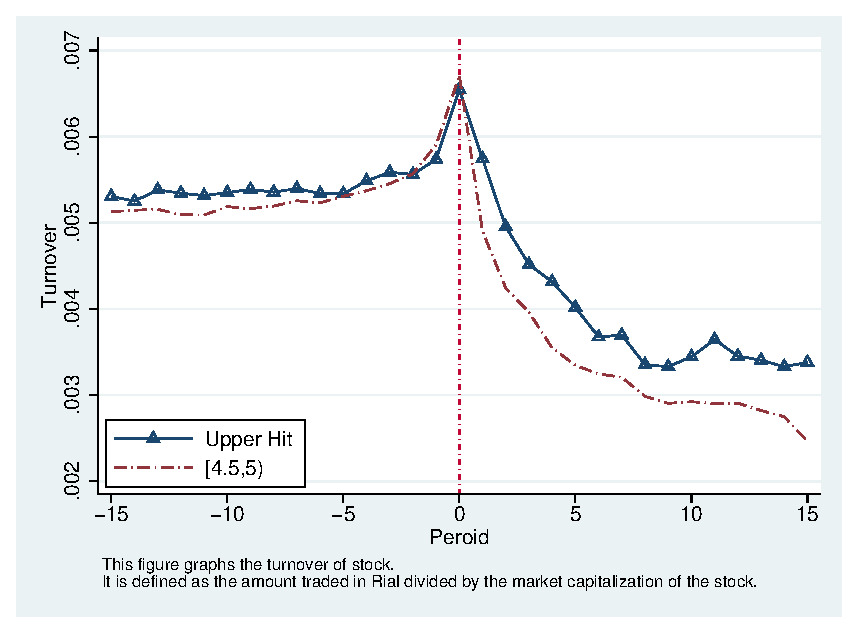
\includegraphics[width=0.7\linewidth]{CUT}
\caption{}
\label{fig:cut}
\end{figure}

\begin{figure}[htbp]
\centering
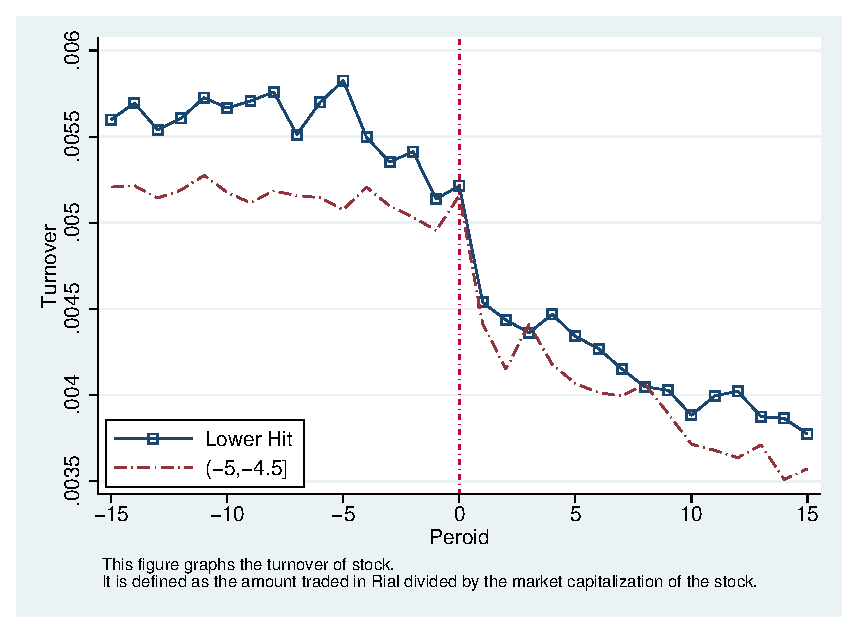
\includegraphics[width=0.7\linewidth]{CLT}
\caption{}
\label{fig:clt}
\end{figure}

\FloatBarrier

‌ % % % % % % % % % % % % % % %
‌ %RT
\subsection{Relative Turnover}
\begin{figure}[htbp]
\centering
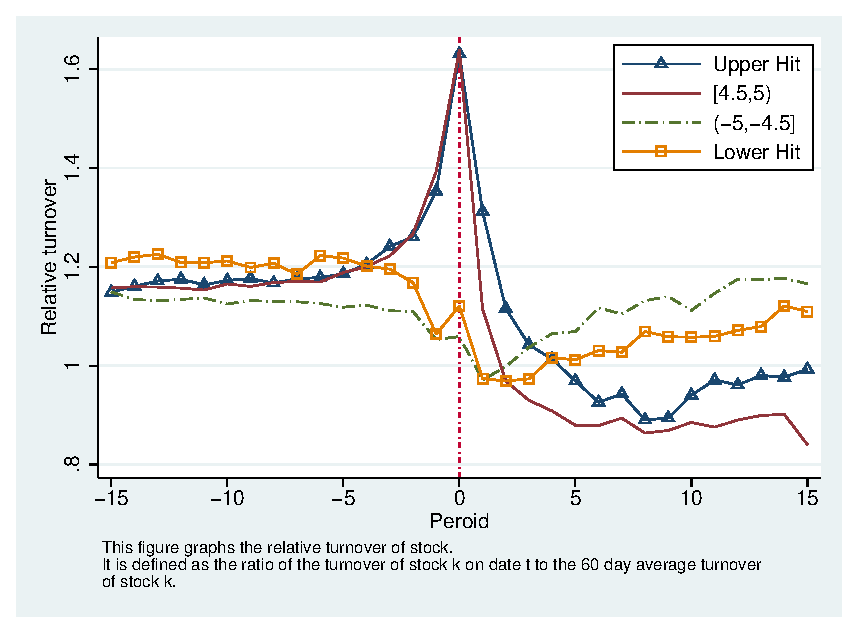
\includegraphics[width=0.7\linewidth]{TRT}
\caption{}
\label{fig:trt}
\end{figure}

\begin{figure}[htbp]
\centering
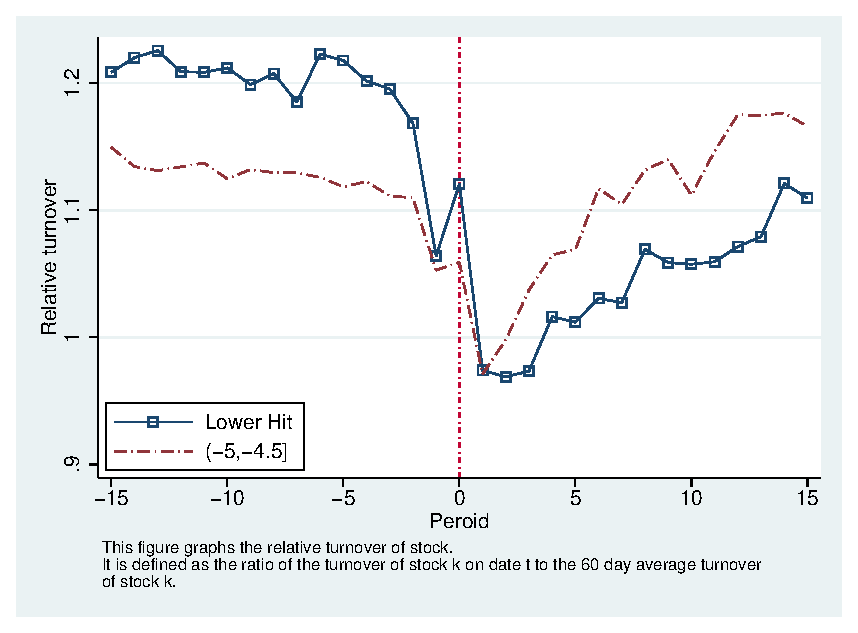
\includegraphics[width=0.7\linewidth]{CLRT}
\caption{}
\label{fig:clrt}
\end{figure}

\begin{figure}[htbp]
\centering
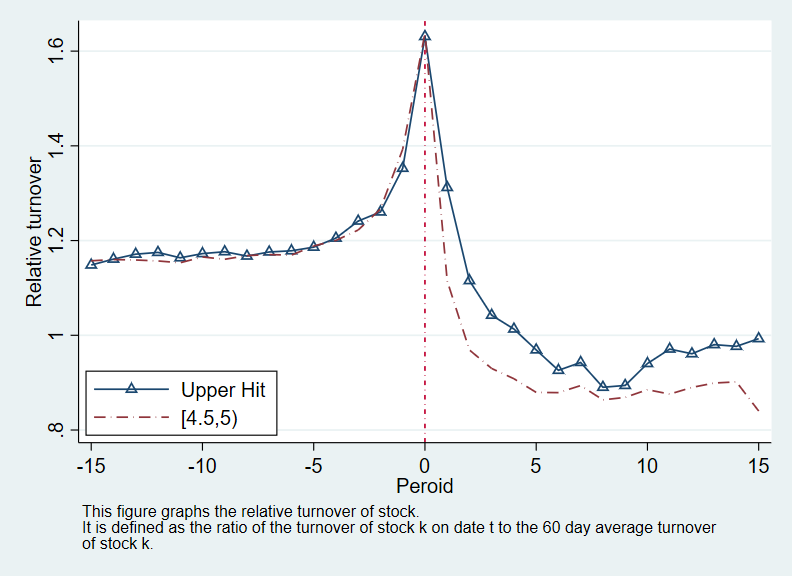
\includegraphics[width=0.7\linewidth]{CURT}
\caption{}
\label{fig:curt}
\end{figure}




\begin{figure}[htbp]
\centering
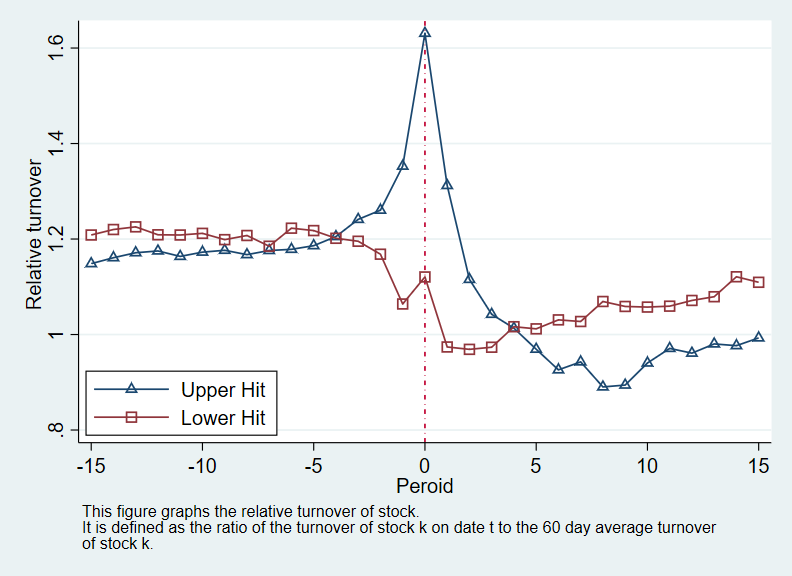
\includegraphics[width=0.7\linewidth]{RT}
\caption{}
\label{fig:rt}
\end{figure}

\begin{figure}[htbp]
\centering
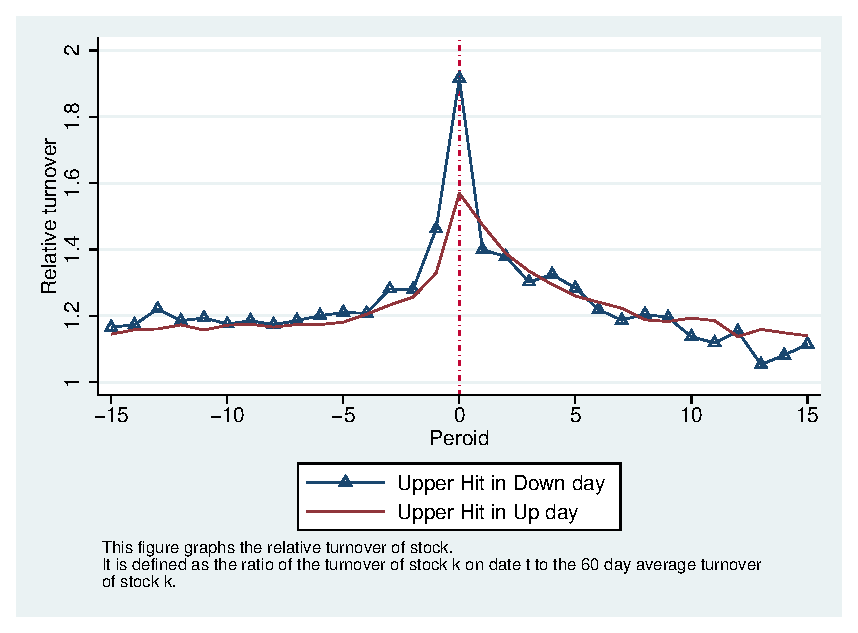
\includegraphics[width=0.7\linewidth]{UPNRT.eps}
\caption{}
\label{fig:UPNRT}
\end{figure}

\begin{figure}[htbp]
\centering
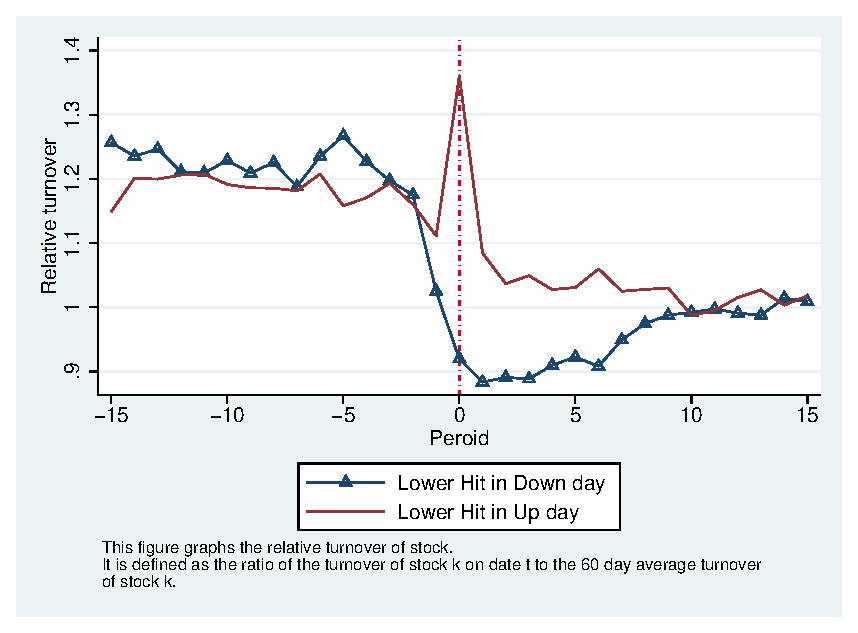
\includegraphics[width=0.7\linewidth]{LPNRT.eps}
\caption{}
\label{fig:LPNRT}
\end{figure}

\begin{figure}[htbp]
\centering
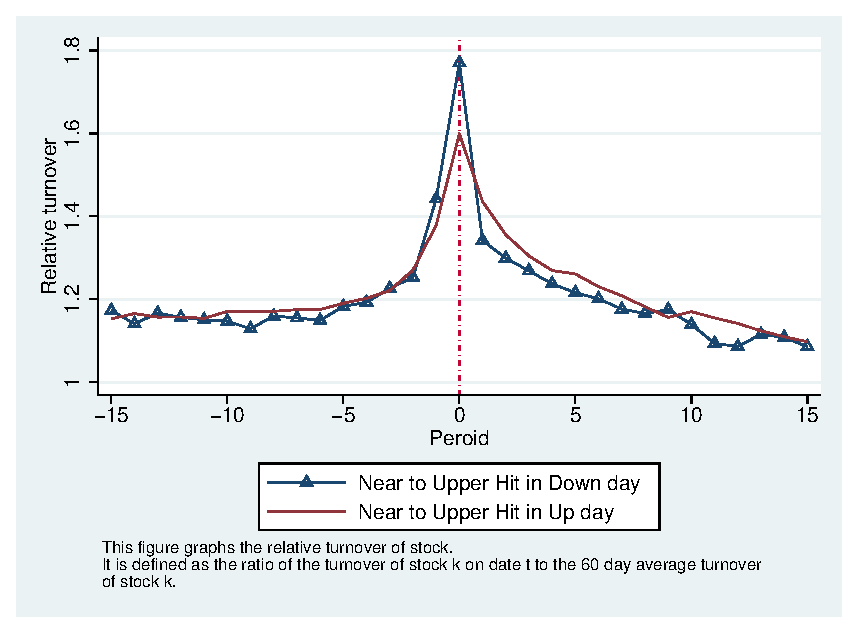
\includegraphics[width=0.7\linewidth]{CUPNRT.eps}
\caption{}
\label{fig:CUPNRT}
\end{figure}

\begin{figure}[htbp]
\centering
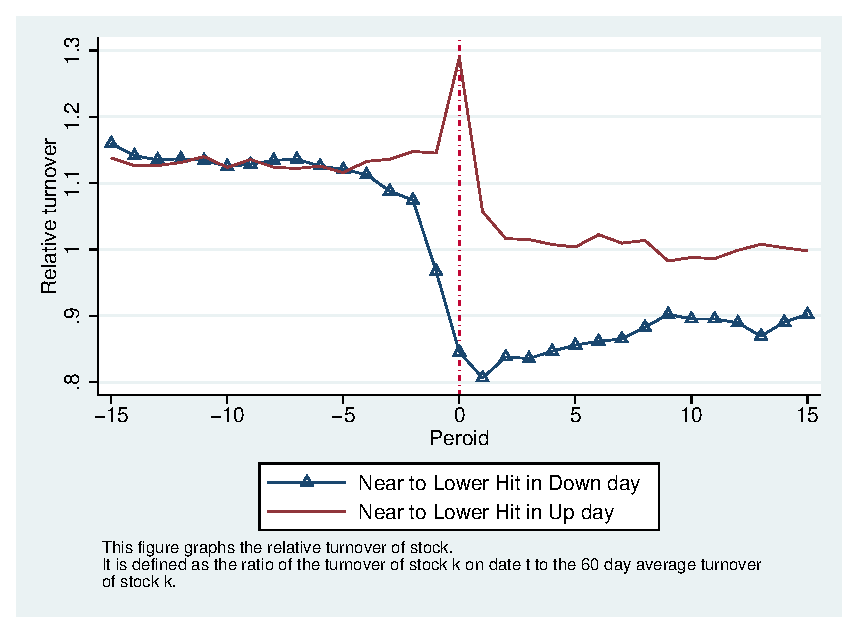
\includegraphics[width=0.7\linewidth]{CLPNRT.eps}
\caption{}
\label{fig:CLPNRT}
\end{figure}

\FloatBarrier
\begin{table}[htbp]
\centering

{{
\def\sym#1{\ifmmode^{#1}\else\(^{#1}\)\fi}
\begin{tabular}{l*{3}{c}}
\hline\hline
                    &\multicolumn{1}{c}{(1)}&\multicolumn{1}{c}{(2)}&\multicolumn{1}{c}{(3)}\\
                    &\multicolumn{1}{c}{lnvolume}&\multicolumn{1}{c}{Turn}&\multicolumn{1}{c}{RelTurn}\\
\hline
upperHit            &       2.179\sym{***}&     0.00636\sym{***}&       1.107\sym{***}\\
                    &     (44.82)         &     (20.34)         &     (49.38)         \\
[1em]
[4.5,5)             &       0.724\sym{***}&     0.00286\sym{***}&       0.599\sym{***}\\
                    &     (37.13)         &     (14.50)         &     (35.42)         \\
[1em]
[4,4.5)             &       0.402\sym{***}&    0.000999\sym{***}&       0.161\sym{***}\\
                    &     (24.09)         &      (8.14)         &     (12.51)         \\
[1em]
[2,4)               &       0.878\sym{***}&     0.00215\sym{***}&       0.288\sym{***}\\
                    &     (31.82)         &     (16.60)         &     (24.34)         \\
[1em]
(-2,2)              &     -0.0289         &     0.00210\sym{***}&      0.0713\sym{***}\\
                    &     (-1.05)         &     (11.53)         &      (4.03)         \\
[1em]
(-4,-2]             &       0.519\sym{***}&     0.00205\sym{***}&       0.144\sym{***}\\
                    &     (28.90)         &     (16.42)         &     (10.31)         \\
[1em]
(-4.5,-4]           &       0.305\sym{***}&     0.00111\sym{***}&      0.0821\sym{***}\\
                    &     (16.63)         &      (4.00)         &      (6.54)         \\
[1em]
(-5,-4.5]           &       0.376\sym{***}&     0.00124\sym{***}&       0.145\sym{***}\\
                    &     (13.39)         &      (4.88)         &     (11.01)         \\
[1em]
lowerHit            &       1.429\sym{***}&     0.00480\sym{***}&       0.514\sym{***}\\
                    &     (37.04)         &     (17.73)         &     (26.49)         \\
[1em]
Up Market           &       0.268\sym{***}&    0.000737\sym{***}&       0.122\sym{***}\\
                    &     (26.43)         &      (6.88)         &     (18.54)         \\
[1em]
Constant            &       12.32\sym{***}&    -0.00120\sym{***}&       0.394\sym{***}\\
                    &    (280.83)         &     (-4.05)         &     (19.25)         \\
\hline
Observations        &      305297         &      305298         &      305298         \\
\(R^{2}\)           &       0.225         &       0.028         &       0.068         \\
\hline\hline
\multicolumn{4}{l}{\footnotesize \textit{t} statistics in parentheses}\\
\multicolumn{4}{l}{\footnotesize This table reports fixed effect estimates of volume, turnover and relative turnover.}\\
\multicolumn{4}{l}{\footnotesize The independent variables are dummies that control for events . We calculate standard errors by using fixed effect on stock level}\\
\multicolumn{4}{l}{\footnotesize \sym{*} \(p<0.05\), \sym{**} \(p<0.01\), \sym{***} \(p<0.001\)}\\
\end{tabular}
}
}
\end{table}



\FloatBarrier


%
%\section{Value}
%
%\begin{figure}[htbp]
%\centering
%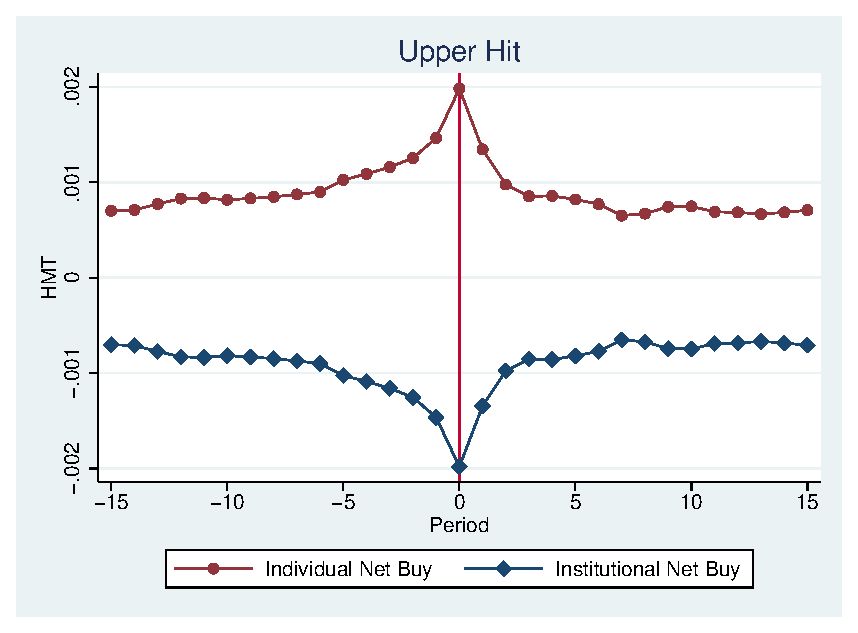
\includegraphics[width=0.7\linewidth]{UV}
%\caption{}
%\label{fig:UV}
%\end{figure}
%\begin{figure}[htbp]
%\centering
%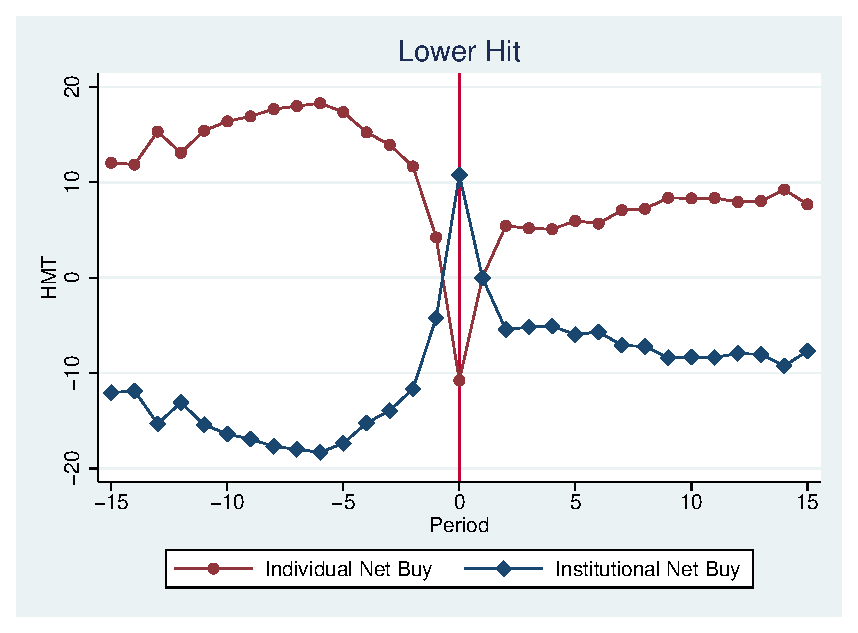
\includegraphics[width=0.7\linewidth]{LV}
%\caption{}
%\label{fig:LV}
%\end{figure}
%\begin{figure}[htbp]
%\centering
%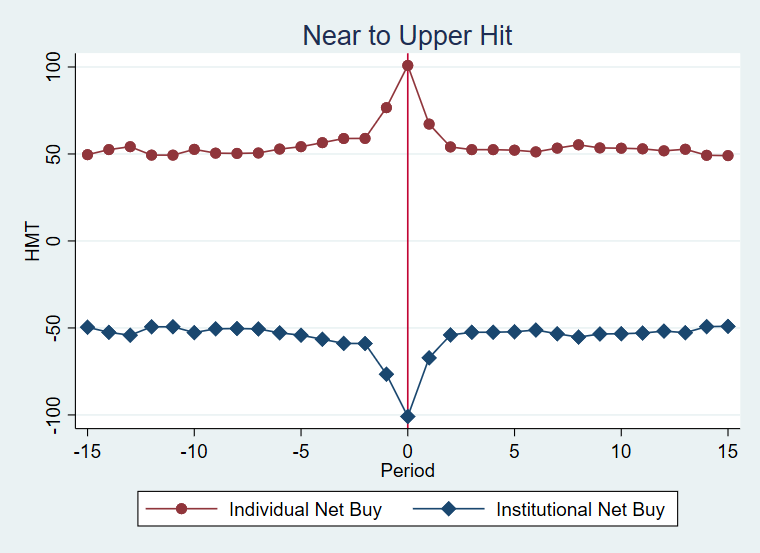
\includegraphics[width=0.7\linewidth]{CUV}
%\caption{}
%\label{fig:CUV}
%\end{figure}
%\begin{figure}[htbp]
%\centering
%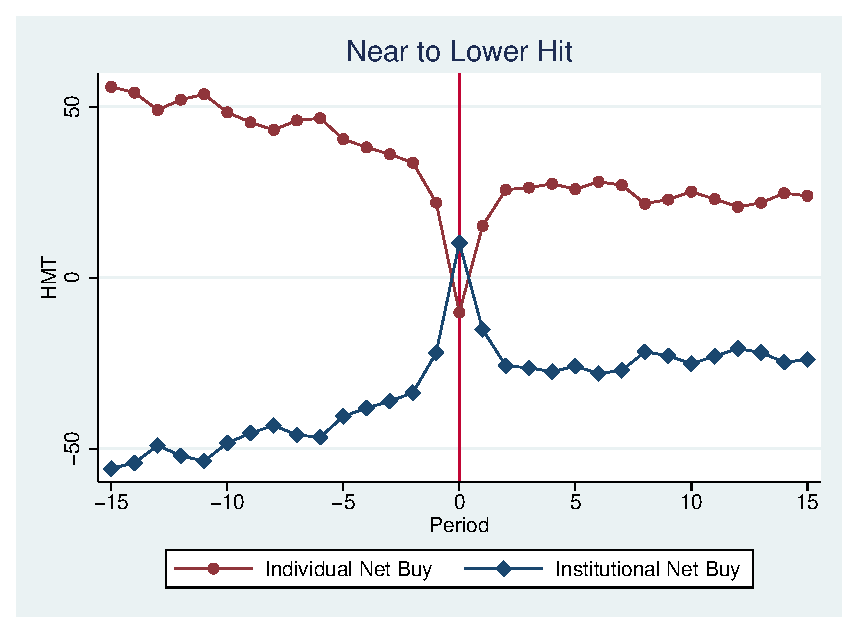
\includegraphics[width=0.7\linewidth]{CLV}
%\caption{}
%\label{fig:CLV}
%\end{figure}
%
%\FloatBarrier
%
%
%
%\begin{figure}[htbp]
%\centering
%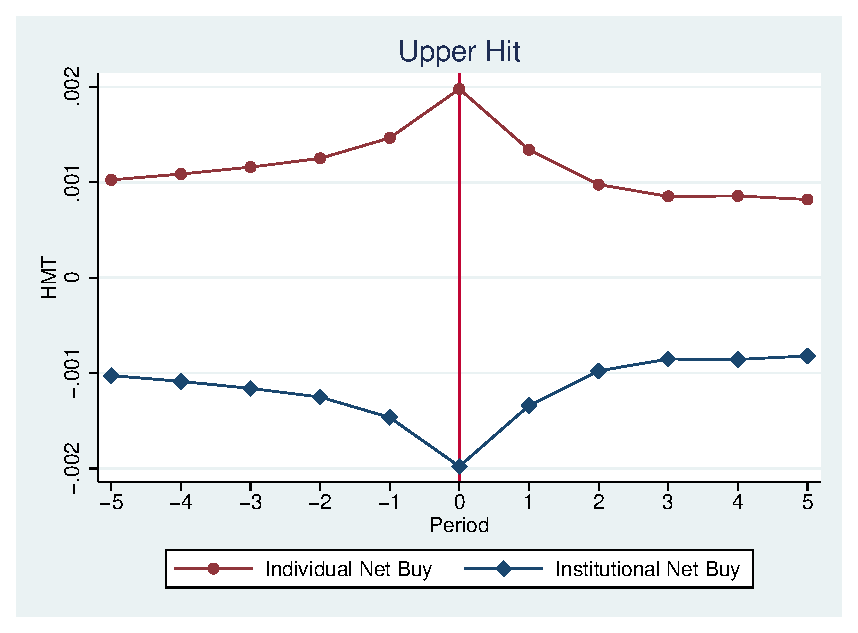
\includegraphics[width=0.7\linewidth]{UV2}
%\caption{}
%\label{fig:UV2}
%\end{figure}
%\begin{figure}[htbp]
%\centering
%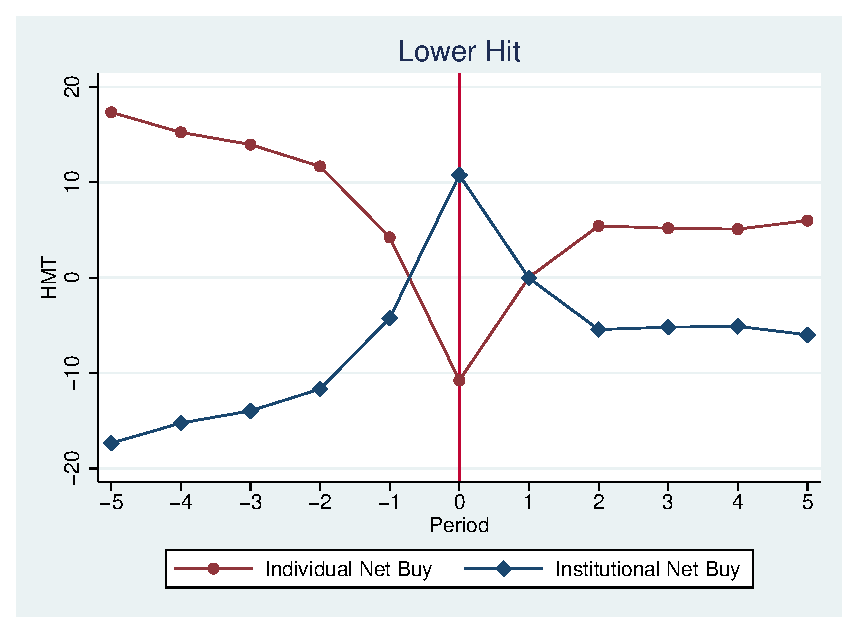
\includegraphics[width=0.7\linewidth]{LV2}
%\caption{}
%\label{fig:LV2}
%\end{figure}
%\begin{figure}[htbp]
%\centering
%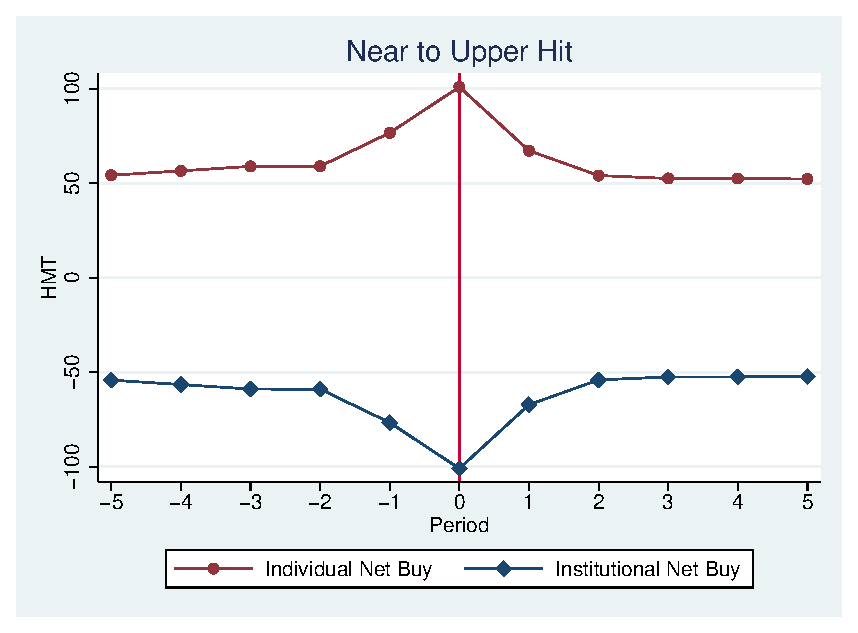
\includegraphics[width=0.7\linewidth]{CUV2}
%\caption{}
%\label{fig:CUV2}
%\end{figure}
%\begin{figure}[htbp]
%\centering
%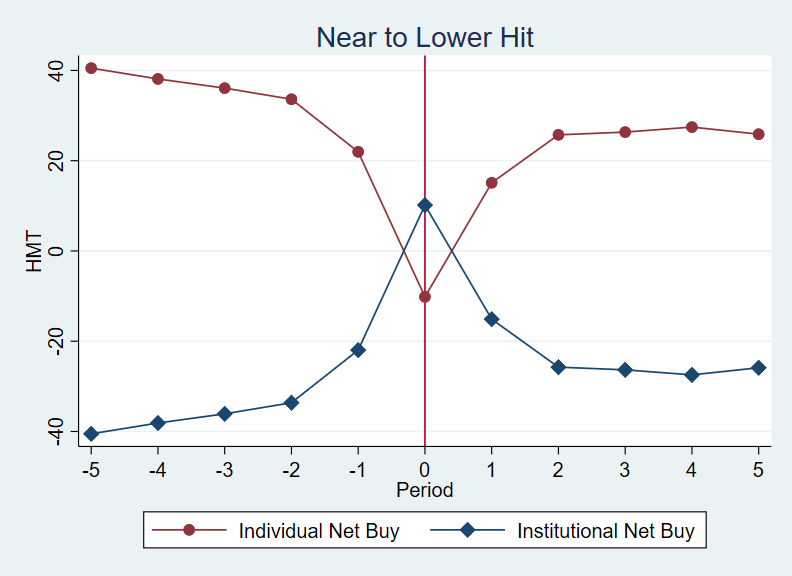
\includegraphics[width=0.7\linewidth]{CLV2}
%\caption{}
%\label{fig:CLV2}
%\end{figure}
%
%\FloatBarrier
%
%
%\begin{figure}[htbp]
%\centering
%\includegraphics[width=0.7\linewidth]{UVCUM}
%\caption{}
%\label{fig:UVCUM}
%\end{figure}
%\begin{figure}[htbp]
%\centering
%\includegraphics[width=0.7\linewidth]{LVCUM}
%\caption{}
%\label{fig:LVCUM}
%\end{figure}
%\begin{figure}[htbp]
%\centering
%\includegraphics[width=0.7\linewidth]{CUVCUM}
%\caption{}
%\label{fig:CUVCUM}
%\end{figure}
%\begin{figure}[htbp]
%\centering
%\includegraphics[width=0.7\linewidth]{CLVCUM}
%\caption{}
%\label{fig:CLVCUM}
%\end{figure}
%
%\FloatBarrier
\begin{appendices}

\section{Extra Return from Market}



‌ % % % % % % % % % % % % % % %
‌ % ER


\begin{figure}[htbp]
\centering
\includegraphics[width=0.7\linewidth]{TER}
\caption{}
\label{fig:ter}
\end{figure}


\begin{figure}[htbp]
\centering
\includegraphics[width=0.7\linewidth]{CUER}
\caption{}
\label{fig:cuer}
\end{figure}


\begin{figure}[htbp]
\centering
\includegraphics[width=0.7\linewidth]{CLER}
\caption{}
\label{fig:cler}
\end{figure}

\begin{figure}[htbp]
\centering
\includegraphics[width=0.7\linewidth]{ER}
\caption{}
\label{fig:er}
\end{figure}

\FloatBarrier
\begin{table}[htbp]
\centering

{{
\def\sym#1{\ifmmode^{#1}\else\(^{#1}\)\fi}
\begin{tabular}{l*{6}{c}}
\hline\hline
                    &\multicolumn{1}{c}{(1)}&\multicolumn{1}{c}{(2)}&\multicolumn{1}{c}{(3)}&\multicolumn{1}{c}{(4)}&\multicolumn{1}{c}{(5)}&\multicolumn{1}{c}{(6)}\\
                    &\multicolumn{1}{c}{ERet\_1}&\multicolumn{1}{c}{ERet\_2}&\multicolumn{1}{c}{E[2,5]}&\multicolumn{1}{c}{E[5,50]}&\multicolumn{1}{c}{E[50,100]}&\multicolumn{1}{c}{E[100,300]}\\
\hline
upperHit            &       1.306\sym{***}&       1.680\sym{***}&       0.357\sym{***}&      -3.365\sym{**} &      -7.211\sym{***}&      -47.00\sym{***}\\
                    &     (42.20)         &     (25.72)         &      (3.64)         &     (-2.82)         &     (-3.52)         &     (-3.39)         \\
[1em]
[4.5,5)             &       0.991\sym{***}&       1.220\sym{***}&      0.0828         &      -5.042\sym{***}&      -7.035\sym{***}&      -8.743         \\
                    &     (29.90)         &     (21.42)         &      (1.05)         &     (-8.09)         &     (-6.33)         &     (-1.50)         \\
[1em]
[4,4.5)             &      -0.153\sym{***}&      -0.317\sym{***}&      -0.209\sym{**} &      -0.437         &      -0.295         &       9.666         \\
                    &     (-5.34)         &     (-6.41)         &     (-2.97)         &     (-0.94)         &     (-0.34)         &      (1.87)         \\
[1em]
[2,4)               &     -0.0536\sym{**} &      0.0377         &       0.277\sym{***}&       1.157\sym{**} &       0.275         &      -1.784         \\
                    &     (-2.62)         &      (0.99)         &      (4.93)         &      (3.20)         &      (0.42)         &     (-0.46)         \\
[1em]
(-2,2)              &      -0.193\sym{***}&      -0.186\sym{***}&     -0.0201         &      -1.766\sym{***}&      -3.092\sym{***}&      -12.93\sym{**} \\
                    &     (-7.74)         &     (-3.83)         &     (-0.28)         &     (-3.39)         &     (-3.72)         &     (-3.01)         \\
[1em]
(-4,-2]             &      -0.476\sym{***}&      -0.559\sym{***}&      -0.192\sym{***}&      -0.444         &      -1.701\sym{**} &      -5.690         \\
                    &    (-22.14)         &    (-14.27)         &     (-3.39)         &     (-1.19)         &     (-2.67)         &     (-1.55)         \\
[1em]
(-4.5,-4]           &      -0.113\sym{***}&      -0.149\sym{**} &      -0.200\sym{**} &      -0.645         &      -0.407         &       2.539         \\
                    &     (-3.48)         &     (-3.12)         &     (-3.08)         &     (-1.40)         &     (-0.56)         &      (0.64)         \\
[1em]
(-5,-4.5]           &      -0.403\sym{***}&      -0.704\sym{***}&      -0.535\sym{***}&      -3.536\sym{***}&      -3.721\sym{***}&       4.567         \\
                    &    (-12.44)         &    (-14.04)         &     (-7.86)         &     (-6.21)         &     (-4.09)         &      (0.96)         \\
[1em]
lowerHit            &      -1.308\sym{***}&      -1.843\sym{***}&      -0.961\sym{***}&      -5.154\sym{***}&      -5.280\sym{**} &      -14.60\sym{*}  \\
                    &    (-40.29)         &    (-29.04)         &    (-10.65)         &     (-5.30)         &     (-2.74)         &     (-2.01)         \\
[1em]
Up Market           &      -0.549\sym{***}&      -0.734\sym{***}&      -0.285\sym{***}&      -2.642\sym{***}&      -3.661\sym{***}&      -19.54\sym{***}\\
                    &    (-40.29)         &    (-32.18)         &     (-9.23)         &    (-10.91)         &     (-9.33)         &    (-10.41)         \\
[1em]
Constant            &       0.503\sym{***}&       0.770\sym{***}&       0.764\sym{***}&       3.683\sym{**} &       7.500\sym{***}&       45.71\sym{***}\\
                    &     (17.56)         &     (13.28)         &      (8.27)         &      (2.90)         &      (3.63)         &      (3.61)         \\
\hline
Observations        &      304849         &      304400         &      303053         &      282856         &      260512         &      174360         \\
\(R^{2}\)           &       0.048         &       0.033         &       0.005         &       0.007         &       0.004         &       0.013         \\
\hline\hline
\multicolumn{7}{l}{\footnotesize \textit{t} statistics in parentheses}\\
\multicolumn{7}{l}{\footnotesize This table reports fixed effect estimates of extra return from market.}\\
\multicolumn{7}{l}{\footnotesize The independent variables are dummies that control for events . We calculate standard errors by using fixed effect on stock level}\\
\multicolumn{7}{l}{\footnotesize \sym{*} \(p<0.05\), \sym{**} \(p<0.01\), \sym{***} \(p<0.001\)}\\
\end{tabular}
}
}
\end{table}



\FloatBarrier

‌ % % % % % % % % % % % % % % %
‌ % R
\section{Return}

\begin{figure}[htbp]
\centering
\includegraphics[width=0.7\linewidth]{TR}
\caption{}
\label{fig:tr}
\end{figure}


\begin{figure}[htbp]
\centering
\includegraphics[width=0.7\linewidth]{R}
\caption{}
\label{fig:r}
\end{figure}


\begin{figure}[htbp]
\centering
\includegraphics[width=0.7\linewidth]{CUR}
\caption{}
\label{fig:cur}
\end{figure}

\begin{figure}[htbp]
\centering
\includegraphics[width=0.7\linewidth]{CLR}
\caption{}
\label{fig:clr}
\end{figure}



















\FloatBarrier
\begin{table}[htbp]
\centering

{{
\def\sym#1{\ifmmode^{#1}\else\(^{#1}\)\fi}
\begin{tabular}{l*{6}{c}}
\hline\hline
                    &\multicolumn{1}{c}{(1)}&\multicolumn{1}{c}{(2)}&\multicolumn{1}{c}{(3)}&\multicolumn{1}{c}{(4)}&\multicolumn{1}{c}{(5)}&\multicolumn{1}{c}{(6)}\\
                    &\multicolumn{1}{c}{Ret\_1}&\multicolumn{1}{c}{Ret\_2}&\multicolumn{1}{c}{[2,5]}&\multicolumn{1}{c}{[5,50]}&\multicolumn{1}{c}{[50,100]}&\multicolumn{1}{c}{[100,300]}\\
\hline
upperHit            &       1.856\sym{***}&       2.732\sym{***}&       1.714\sym{***}&       20.44\sym{***}&       8.055\sym{***}&       117.4\sym{***}\\
                    &     (60.81)         &     (41.73)         &     (17.21)         &     (17.28)         &      (3.38)         &      (7.71)         \\
[1em]
[4.5,5)             &       1.269\sym{***}&       1.703\sym{***}&       0.696\sym{***}&       0.223         &       1.873         &      -10.31         \\
                    &     (38.33)         &     (30.29)         &      (8.50)         &      (0.32)         &      (1.54)         &     (-1.51)         \\
[1em]
[4,4.5)             &     -0.0932\sym{**} &      -0.196\sym{***}&     -0.0282         &       2.060\sym{***}&       3.051\sym{**} &       30.31\sym{***}\\
                    &     (-3.13)         &     (-3.97)         &     (-0.39)         &      (3.88)         &      (3.24)         &      (5.07)         \\
[1em]
[2,4)               &     -0.0102         &       0.141\sym{***}&       0.532\sym{***}&       5.174\sym{***}&       8.859\sym{***}&       43.64\sym{***}\\
                    &     (-0.51)         &      (3.78)         &      (9.43)         &     (13.34)         &     (12.44)         &      (9.37)         \\
[1em]
(-2,2)              &      -0.230\sym{***}&      -0.170\sym{***}&     -0.0426         &      -2.881\sym{***}&       1.380         &      -13.45\sym{**} \\
                    &     (-9.33)         &     (-3.44)         &     (-0.57)         &     (-5.10)         &      (1.43)         &     (-2.63)         \\
[1em]
(-4,-2]             &      -0.491\sym{***}&      -0.562\sym{***}&      -0.122\sym{*}  &       2.454\sym{***}&       6.004\sym{***}&       21.34\sym{***}\\
                    &    (-22.94)         &    (-13.72)         &     (-2.07)         &      (6.27)         &      (8.93)         &      (4.90)         \\
[1em]
(-4.5,-4]           &     -0.0236         &     0.00775         &     -0.0253         &       2.317\sym{***}&       1.121         &       15.28\sym{**} \\
                    &     (-0.78)         &      (0.16)         &     (-0.37)         &      (4.50)         &      (1.42)         &      (3.08)         \\
[1em]
(-5,-4.5]           &      -0.564\sym{***}&      -0.908\sym{***}&      -0.669\sym{***}&      -0.485         &       2.315\sym{*}  &      -7.919         \\
                    &    (-18.13)         &    (-17.76)         &     (-9.23)         &     (-0.76)         &      (2.37)         &     (-1.49)         \\
[1em]
lowerHit            &      -1.333\sym{***}&      -1.781\sym{***}&      -0.609\sym{***}&       8.191\sym{***}&       13.20\sym{***}&       28.82\sym{**} \\
                    &    (-42.83)         &    (-28.01)         &     (-6.26)         &      (7.56)         &      (6.16)         &      (3.17)         \\
[1em]
Up Market           &      0.0615\sym{***}&    -0.00688         &       0.129\sym{***}&       0.831\sym{***}&       3.174\sym{***}&      -9.868\sym{***}\\
                    &      (5.09)         &     (-0.33)         &      (4.57)         &      (3.56)         &      (8.07)         &     (-4.80)         \\
[1em]
Constant            &       0.394\sym{***}&       0.892\sym{***}&       1.445\sym{***}&       26.24\sym{***}&       41.06\sym{***}&       313.2\sym{***}\\
                    &     (14.82)         &     (15.47)         &     (15.28)         &     (16.55)         &     (15.74)         &     (20.68)         \\
\hline
Observations        &      304849         &      304400         &      303053         &      282856         &      260512         &      174360         \\
\(R^{2}\)           &       0.082         &       0.060         &       0.014         &       0.032         &       0.017         &       0.019         \\
\hline\hline
\multicolumn{7}{l}{\footnotesize \textit{t} statistics in parentheses}\\
\multicolumn{7}{l}{\footnotesize This table reports fixed effect estimates of normal returns.}\\
\multicolumn{7}{l}{\footnotesize The independent variables are dummies that control for events . We calculate standard errors by using fixed effect on stock level}\\
\multicolumn{7}{l}{\footnotesize \sym{*} \(p<0.05\), \sym{**} \(p<0.01\), \sym{***} \(p<0.001\)}\\
\end{tabular}
}
}
\end{table}

\end{appendices}

\end{document}